\clearpage
\section{Stokes 方程的离散化 (II)}
\label{sec:ch1-stokes-discretization-ii}

本节研究用有限元方法离散化 Stokes 方程. 这里的结果不如上一节一般, 并随维数而变化. 我们依次考虑下列协调有限元: 二维情形下的分片二次多项式, 三维情形下的分片三次多项式, 以及二维情形下的分片四次多项式. 最后考虑由非协调有限元给出的外逼近, 这适用于任意维数.

\subsection{预备结果}
\label{subsec:ch1-finite-element-preliminaries}

我们将使用定义在 $n$-单纯形上的分片多项式函数. 为此, 先回顾一些定义并引入适合当前情形的记号.

\subsubsection*{重心坐标}

设在 $\mathbb R^n$ 中给定 $n+1$ 个点 $A_1,\ldots,A_{n+1}$, 其坐标为 $a_{1,i},\ldots,a_{n,i}$, $1\leq i\leq n+1$, 且这些点不在同一超平面上. 这等价于 $n$ 个向量 $A_1A_2,\ldots,A_1A_{n+1}$ 线性无关, 也等价于矩阵
\begin{equation}
\mathcal A=
\begin{pmatrix}
a_{1,1}&a_{1,2}&\cdots&a_{1,n+1}\\
a_{2,1}&a_{2,2}&\cdots&a_{2,n+1}\\
\vdots&\vdots&&\vdots\\
a_{n,1}&a_{n,2}&\cdots&a_{n,n+1}\\
1&1&\cdots&1
\end{pmatrix}
\label{eq:ch1-simplex-coordinate-matrix}
\end{equation}
非奇异.

给定坐标为 $x_1,\ldots,x_n$ 的任意点 $P\in\mathbb R^n$, 存在 $n+1$ 个实数 $\lambda_i=\lambda_i(P)$, $1\leq i\leq n+1$, 使
\begin{equation}
OP=\sum_{i=1}^{n+1}\lambda_iOA_i,
\label{eq:ch1-barycentric-position}
\end{equation}
\begin{equation}
\sum_{i=1}^{n+1}\lambda_i=1,
\label{eq:ch1-barycentric-sum}
\end{equation}
其中 $O$ 是 $\mathbb R^n$ 的原点.

只需注意, \eqref{eq:ch1-barycentric-position} 与 \eqref{eq:ch1-barycentric-sum} 等价于线性方程组
\begin{equation}
\mathcal A
\begin{pmatrix}
\lambda_1\\ \vdots\\ \lambda_n\\ \lambda_{n+1}
\end{pmatrix}
=
\begin{pmatrix}
x_1\\ \vdots\\ x_n\\ 1
\end{pmatrix},
\label{eq:ch1-barycentric-linear-system}
\end{equation}
而按假设矩阵 $\mathcal A$ 非奇异, 所以该方程组有唯一解. 数 $\lambda_i$ 称为 $P$ 关于 $n+1$ 个点 $A_1,\ldots,A_{n+1}$ 的重心坐标.

由 \eqref{eq:ch1-barycentric-linear-system}, $\lambda_i$ 是 $P$ 的坐标 $x_1,\ldots,x_n$ 的线性函数, 一般是非齐次的:
\begin{equation}
\lambda_i=\sum_{j=1}^nb_{i,j}x_j+b_{i,n+1},
\qquad1\leq i\leq n+1,
\label{eq:ch1-barycentric-affine-functions}
\end{equation}
其中矩阵 $\mathcal B=(b_{i,j})$ 是矩阵 $\mathcal A$ 的逆. 容易看出, 在 \eqref{eq:ch1-barycentric-position} 中把点 $O$ 换成 $\mathbb R^n$ 中另一点不会改变重心坐标的值; 因而
\begin{equation}
\sum_{i=1}^{n+1}\lambda_iPA_i=0.
\label{eq:ch1-barycentric-vector-identity}
\end{equation}

$n+1$ 个点 $A_i$ 的凸包恰为重心坐标满足下列条件的点集:
\begin{equation}
0\leq\lambda_i\leq1,\qquad1\leq i\leq n+1.
\label{eq:ch1-simplex-barycentric-bounds}
\end{equation}
这个凸包 $S$ 是由点 $A_i$ 生成的 $n$-单纯形, 这些点称为该 $n$-单纯形的顶点. $S$ 的重心 $G$ 是 $S$ 中所有重心坐标都等于 $1/(n+1)$ 的点. $S$ 的一个 $m$ 维面是由 $S$ 的 $m+1$ 个顶点生成的任意 $m$-单纯形, 其中 $1\leq m\leq n-1$. 一维面称为边.

在二维情形($n=1$)下, 2-单纯形是三角形. 在三维情形下, 3-单纯形是四面体, 二维面是构成其边界的四个三角形.

\MBSourceStatementNumber{proposition}{1}
\begin{Proposition}
\label{prop:ch1-linear-barycentric-interpolation}
设 $A_1,\ldots,A_{n+1}$ 是 $\mathbb R^n$ 中不包含于同一超平面的 $n+1$ 个点. 给定 $n+1$ 个实数 $\alpha_1,\ldots,\alpha_{n+1}$, 存在唯一线性函数 $u$, 使 $u(A_i)=\alpha_i$, 并且
\begin{equation}
u(P)=\sum_{i=1}^{n+1}\alpha_i\lambda_i(P),
\qquad\forall P\in\mathbb R^n.
\label{eq:ch1-linear-barycentric-interpolation}
\end{equation}
\end{Proposition}

\begin{Proof}
令 $u(x)=\sum_{j=1}^n\beta_jx_j+\beta_{n+1}$. 未知数满足
\[
\sum_{j=1}^n\beta_ja_{j,i}+\beta_{n+1}=\alpha_i,
\qquad1\leq i\leq n+1.
\]
方程组的矩阵是 $\mathcal A$ 的转置矩阵, 因而函数 $u$ 存在且唯一. 公式 \eqref{eq:ch1-linear-barycentric-interpolation} 给出该函数, 因为 $\lambda_i(A_j)=\delta_{ij}$.
\end{Proof}

\MBSourceStatementNumber{remark}{1}
\begin{Remark}
\label{rem:ch1-higher-order-barycentric-interpolation}
稍后将给出使用重心坐标的高阶插值公式.
\end{Remark}

\subsubsection*{微分性质}

下面给出把 $\lambda_i$ 看作点 $P$ 的 Cartesian 坐标函数时所具有的一些微分性质; 用 $D$ 表示梯度算子 $D=(D_1,\ldots,D_n)$.

\MBSourceStatementNumber{lemma}{1}
\begin{Lemma}
\label{lem:ch1-barycentric-differential-identities}
\begin{equation}
\sum_{i=1}^{n+1}D\lambda_i=0,
\label{eq:ch1-barycentric-gradient-sum}
\end{equation}
\begin{equation}
D\lambda_i(P)\cdot PA_j=\delta_{ij}-\lambda_i(P),
\qquad1\leq i,j\leq n+1.
\label{eq:ch1-barycentric-gradient-vector}
\end{equation}
\end{Lemma}

\begin{Proof}
\eqref{eq:ch1-barycentric-sum} 立即蕴含 \eqref{eq:ch1-barycentric-gradient-sum}. 由 \eqref{eq:ch1-barycentric-affine-functions},
\[
\frac{\partial\lambda_i}{\partial x_k}=b_{i,k}.
\]
于是
\[
\begin{aligned}
D\lambda_i(P)\cdot PA_j
&=D\lambda_i(P)\cdot OA_j-D\lambda_i(P)\cdot OP\\
&=\sum_{k=1}^nb_{i,k}a_{k,j}-\sum_{k=1}^nb_{i,k}x_k\\
&=\sum_{k=1}^nb_{i,k}a_{k,j}+b_{i,n+1}-\lambda_i
=\delta_{ij}-\lambda_i.
\end{aligned}
\]
\end{Proof}

\MBSourceStatementNumber{lemma}{2}
\begin{Lemma}
\label{lem:ch1-barycentric-gradient-bound}
设 $S$ 是顶点为 $A_1,\ldots,A_{n+1}$ 的 $n$-单纯形, $\rho'$ 是 $S$ 中所含全部球的直径的最小上界. 则
\begin{equation}
|D\lambda_i|\leq\frac1{\rho'},
\qquad1\leq i\leq n+1.
\label{eq:ch1-barycentric-gradient-bound}
\end{equation}
\end{Lemma}

\begin{Proof}
有
\begin{equation}
|D\lambda_i|=D\lambda_i\cdot x,
\label{eq:ch1-barycentric-gradient-direction}
\end{equation}
其中 $x$ 是与 $D\lambda_i$ 平行的单位向量. 可写成 $x=PQ/\rho'$, 其中 $P,Q\in S$. 以 $\mu_j$ 表示 $Q$ 的重心坐标, 则
\[
PQ=\sum_{j=1}^{n+1}\mu_jPA_j,\qquad
\sum_{j=1}^{n+1}\mu_j=1.
\]
因此, 由 \eqref{eq:ch1-barycentric-gradient-vector},
\[
D\lambda_i\cdot x
=\frac1{\rho'}\sum_{j=1}^{n+1}\mu_j(\delta_{ij}-\lambda_i)
=\frac1{\rho'}(\mu_i-\lambda_i).
\]
因为 $P,Q\in S$, 有 $-1\leq\mu_i-\lambda_i\leq1$, 从而得到 \eqref{eq:ch1-barycentric-gradient-bound}.
\end{Proof}

\subsubsection*{若干线性变换的范数}

设 $S$ 和 $\overline S$ 是两个 $n$-单纯形. 以 $\rho$(相应地 $\rho'$)表示包含 $S$ 的最小球的直径(相应地 $S$ 中所含最大球的直径); $\overline\rho,\overline\rho'$ 具有类似含义.

经过平移后可设相应的第一个顶点都为原点. 以 $\Lambda$ 表示满足
\begin{equation}
A_i=\Lambda\overline A_i,\qquad1\leq i\leq n+1,
\label{eq:ch1-simplex-linear-map}
\end{equation}
的线性映射.

\MBSourceStatementNumber{lemma}{3}
\begin{Lemma}
\label{lem:ch1-simplex-linear-map-norms}
\begin{equation}
\|\Lambda\|\leq\frac{\overline\rho}{\rho'},
\qquad
\|\Lambda^{-1}\|\leq\frac{\rho}{\overline\rho'}.
\label{eq:ch1-simplex-linear-map-norms}
\end{equation}
\end{Lemma}

\begin{Proof}
如引理 \ref{lem:ch1-barycentric-gradient-bound} 的证明, 令 $x$ 是任意单位向量, 写成 $x=PQ/\rho'$, 其中 $P,Q\in S$. 则
\[
\Lambda x=\frac1{\rho'}\overline P\,\overline Q,
\]
其中 $\overline P=\Lambda P$, $\overline Q=\Lambda Q$. 点 $\overline P,\overline Q$ 属于 $\overline S$, 因为线性映射保持相应的重心坐标. 因而
\[
|\Lambda x|\leq\frac{\overline\rho}{\rho'}.
\]
这证明第一个不等式. 交换 $S$ 与 $\overline S$ 的角色即可得到第二个不等式.
\end{Proof}

\MBSourceStatementNumber{lemma}{4}
\begin{Lemma}
\label{lem:ch1-linear-map-preserves-divergence}
设 $x\mapsto u(x)$ 是定义在 $S$ 上的无散向量函数, 并在 $\overline S$ 上定义
\begin{equation}
\overline u(\overline x)=\Lambda u(\Lambda^{-1}\overline x),
\qquad\forall\overline x\in\overline S.
\label{eq:ch1-divergence-preserving-transform}
\end{equation}
则 $\overline u$ 也是无散向量函数.
\end{Lemma}

\begin{Proof}
以 $(\alpha_{ij})$ 和 $(\beta_{k\ell})$ 分别表示 $\Lambda$ 与 $\Lambda^{-1}$ 的元素. 则
\[
\frac{\partial\overline u_i}{\partial\overline x_j}(\overline x)
=\sum_{\ell,k}\alpha_{i\ell}\beta_{kj}
\frac{\partial u_\ell}{\partial x_k}(\Lambda^{-1}\overline x),
\]
从而
\[
(\operatorname{div}\overline u)(\overline x)
=\sum_{i,k,\ell}\alpha_{i\ell}\beta_{ki}
\frac{\partial u_\ell}{\partial x_k}(\Lambda^{-1}\overline x)
=\sum_k\frac{\partial u_k}{\partial x_k}(\Lambda^{-1}\overline x)=0.
\]
\end{Proof}

\subsubsection*{开集 $\Omega$ 的正则剖分}

设 $\Omega$ 是 $\mathbb R^n$ 中有界开集. 设 $T_h$ 是一族 $n$-单纯形. 若满足下列条件, 则称这样的族为 $\Omega$ 的一个容许剖分:
\begin{equation}
\Omega(h)=\bigcup_{S\in T_h}S\subset\Omega,
\label{eq:ch1-triangulation-covered-domain}
\end{equation}
\begin{equation}
\begin{gathered}
\text{若 }S,S'\in T_h,\text{ 则 }\mathring S\cap\mathring S'=\varnothing,\\
\text{并且 }S\cap S'\text{ 或为空, 或恰为二者的同一个完整 }m\text{ 维面},\\
0\leq m\leq n-1.
\end{gathered}
\label{eq:ch1-admissible-triangulation-intersections}
\end{equation}

以 $\{T_h\}_{h\in\mathcal H}$ 表示 $\Omega$ 的全部容许剖分族; 对每个容许剖分 $T_h$, 联系下列三个数:
\begin{equation}
\rho(h)=\sup_{S\in T_h}\rho_S,
\label{eq:ch1-triangulation-max-diameter}
\end{equation}
\begin{equation}
\rho'(h)=\sup_{S\in T_h}\rho'_S,
\label{eq:ch1-triangulation-max-inscribed-diameter}
\end{equation}
\begin{equation}
\sigma(h)=\sup_{S\in T_h}\frac{\rho_S}{\rho'_S}.
\label{eq:ch1-triangulation-shape-ratio}
\end{equation}

在有限元方法中, 我们关心的是 $\rho(h)\to0$ 的极限过程. 若当 $\rho(h)\to0$ 时 $\sigma(h)$ 保持有界, 则称该容许剖分子族为 $\Omega$ 的正则剖分:
\begin{equation}
\sigma(h)\leq\alpha<+\infty,\qquad\rho(h)\to0,
\label{eq:ch1-regular-triangulation-shape-bound}
\end{equation}
并且 $\Omega(h)$ 按下列意义收敛到 $\Omega$:
\begin{equation}
\begin{gathered}
\text{对每个紧集 }K\subset\Omega,\text{ 存在 }\delta=\delta(K)>0,\text{ 使}\\
\rho(h)\leq\delta(K)\quad\Longrightarrow\quad\Omega(h)\supset K.
\end{gathered}
\label{eq:ch1-triangulation-domain-exhaustion}
\end{equation}
以 $\mathcal H_\alpha$ 表示满足 \eqref{eq:ch1-regular-triangulation-shape-bound} 和 \eqref{eq:ch1-triangulation-domain-exhaustion} 的容许剖分集合.

\MBSourceStatementNumber{remark}{2}
\begin{Remark}
\label{rem:ch1-triangle-minimum-angle}
在二维情形中, 2-单纯形是三角形, 并且
\[
\frac1{2\tan(\theta/2)}
\leq\frac{\rho_S}{\rho'_S}
\leq\frac2{\sin\theta},
\]
其中 $\theta$ 是 $S$ 的最小角. 因而条件 \eqref{eq:ch1-regular-triangulation-shape-bound} 等价于说所有三角形的最小角都有一致正下界:
\begin{equation}
\theta\geq\theta_0>0.
\label{eq:ch1-triangle-minimum-angle-bound}
\end{equation}
\end{Remark}

现在的目标是, 对 $\Omega$ 的正则剖分族 $\{T_h\}_{h\in\mathcal H_\alpha}$, 联系我们所关心的函数空间的各种逼近.

\subsection{\texorpdfstring{二次有限元 ($n=2$)}{二次有限元 (n=2)}}
\label{subsec:ch1-degree-two-elements}

设 $\Omega$ 是 $\mathbb R^n$ 中有界 Lipschitz 开集. 先描述 $H_0^1(\Omega)$ 的内逼近(任意 $n$), 再描述 $V$ 的外逼近(仅 $n=2$). 逼近函数是分片二次多项式.

\subsubsection{\texorpdfstring{$H_0^1(\Omega)$}{H01(Omega)} 的逼近}
\label{subsubsec:ch1-degree-two-h01}

设 $T_h$ 是 $\Omega$ 的任意容许剖分.

\emph{空间 $W_h$.} 它是连续向量函数空间, 这些函数在
\begin{equation}
\Omega(h)=\bigcup_{S\in T_h}S
\label{eq:ch1-degree-two-domain}
\end{equation}
外为零, 且其每个分量在每个单纯形 $S\in T_h$ 上都是二次多项式. 这里及下文所谓二次多项式, 是指次数不超过二的多项式.

$W_h$ 是 $H_0^1(\Omega)$ 的有限维子空间. 赋予它由 $H_0^1(\Omega)$ 诱导的标量积:
\begin{equation}
((u_h,v_h))_h=((u_h,v_h)),
\qquad\forall u_h,v_h\in W_h.
\label{eq:ch1-degree-two-h01-product}
\end{equation}

\emph{$W_h$ 的一组基.} 若 $S$ 是 $n$-单纯形, 顶点记作 $A_1,\ldots,A_{n+1}$; 以 $A_{ij}$ 表示 $A_iA_j$ 的中点.

\MBSourceStatementNumber{lemma}{5}
\begin{Lemma}
\label{lem:ch1-quadratic-simplex-interpolation}
次数不超过二的多项式由其在点 $A_i,A_{ij}$($1\leq i,j\leq n+1$)处的值唯一确定. 而且, 用关于 $A_1,\ldots,A_{n+1}$ 的重心坐标可写为
\begin{equation}
\varphi(x)
=\sum_{i=1}^{n+1}\left(2\lambda_i(x)^2-\lambda_i(x)\right)\varphi(A_i)
+2\sum_{\substack{i,j=1\\i\neq j}}^{n+1}
\lambda_i(x)\lambda_j(x)\varphi(A_{ij}).
\label{eq:ch1-quadratic-barycentric-interpolation}
\end{equation}
\end{Lemma}

\begin{Proof}
\eqref{eq:ch1-quadratic-barycentric-interpolation} 右端是二次多项式. 若以 $\psi$ 表示该函数, 则
\[
\psi(A_k)=\varphi(A_k),\qquad
\psi(A_{k\ell})=\varphi(A_{k\ell}),
\]
因为 $\lambda_i(A_k)=\delta_{ik}$ 且
$\lambda_i(A_{k\ell})=(\delta_{ik}+\delta_{i\ell})/2$.

二次多项式具有形式
\begin{equation}
\varphi(x)=\alpha_0+\sum_{i=1}^n(\alpha_ix_i+\beta_ix_i^2)
+\sum_{\substack{i,j=1\\i<j}}^n\alpha_{ij}x_ix_j,
\label{eq:ch1-general-quadratic-polynomial}
\end{equation}
由 $(n+1)(n+2)/2$ 个未知系数确定. 点 $A_i$ 有 $n+1$ 个, 点 $A_{ij}$ 有 $n(n+1)/2$ 个, 因而条件
\begin{equation}
\varphi(A_i)=\text{给定值},\qquad
\varphi(A_{ij})=\text{给定值}
\label{eq:ch1-quadratic-interpolation-data}
\end{equation}
恰为关于这些系数的 $(n+1)(n+2)/2$ 个线性方程. 由 \eqref{eq:ch1-quadratic-barycentric-interpolation}, 对任意数据该方程组都有解, 所以方程组正则, 且该解唯一.
\end{Proof}

以 $U_h$ 表示剖分中各单纯形的顶点与边中点的集合, 以 $\mathring U_h$ 表示其中属于 $\Omega(h)$ 内部的点.

\MBSourceStatementNumber{lemma}{6}
\begin{Lemma}
\label{lem:ch1-global-quadratic-interpolant}
存在唯一函数 $u_h\in W_h$, 它在各点 $M\in\mathring U_h$ 取任意给定值.
\end{Lemma}

\begin{Proof}
唯一性已由引理 \ref{lem:ch1-quadratic-simplex-interpolation} 给出. 同一引理还逐个单纯形给出分量为二次多项式的函数 $u_h$, 它在 $\mathring U_h$ 取给定值, 在 $U_h-\mathring U_h$ 以及 $\Omega(h)$ 外为零.

只需验证连续性. 在任意单纯形的每个 $n-1$ 维面上, $u_h$ 每个分量从相邻两侧给出两个次数不超过二的多项式, 它们在该面的顶点与边中点处相等. 把引理 \ref{lem:ch1-quadratic-simplex-interpolation} 应用于 $n-1$ 维单纯形, 可知两侧多项式在整个面上相等, 故 $u_h$ 连续并属于 $W_h$.
\end{Proof}

对每个 $M\in\mathring U_h$, 以 $w_{hM}$ 表示在各单纯形上为二次多项式、在 $\Omega(h)$ 外为零并满足
\begin{equation}
w_{hM}(M)=1,\qquad
w_{hM}(P)=0,\quad\forall P\in\mathring U_h,\ P\neq M
\label{eq:ch1-quadratic-nodal-basis-function}
\end{equation}
的唯一连续标量函数.

\MBSourceStatementNumber{lemma}{7}
\begin{Lemma}
\label{lem:ch1-quadratic-wh-basis}
函数 $w_{hM}e_i$, $M\in\mathring U_h$, $i=1,\ldots,n$, 构成 $W_h$ 的一组基. $W_h$ 的维数为 $nN(h)$, 其中 $N(h)$ 是 $\mathring U_h$ 中点的数目.
\end{Lemma}

\begin{Proof}
这些函数线性无关, 且每个 $u_h\in W_h$ 可写成
\[
u_h(x)=\sum_{M\in\mathring U_h}\sum_{i=1}^nu_{ih}(M)e_iw_{hM}(x),
\]
即
\begin{equation}
u_h=\sum_{M\in\mathring U_h}u_h(M)w_{hM}.
\label{eq:ch1-quadratic-wh-expansion}
\end{equation}
\end{Proof}

\emph{算子 $p_h$.} 延拓算子是恒等算子:
\begin{equation}
p_hu_h=u_h,\qquad\forall u_h\in W_h.
\label{eq:ch1-quadratic-prolongation}
\end{equation}
它们的范数为 $1$, 因而稳定.

\emph{算子 $r_h$.} 对 $u\in\mathcal D(\Omega)$, 定义
\begin{equation}
(r_hu)(M)=u(M),\qquad\forall M\in\mathring U_h.
\label{eq:ch1-quadratic-restriction}
\end{equation}

\MBSourceStatementNumber{proposition}{2}
\begin{Proposition}
\label{prop:ch1-quadratic-h01-convergence}
若 $h$ 属于 $\Omega$ 的正则剖分 $\mathcal H_\alpha$, 则上述 $H_0^1(\Omega)$ 的内逼近稳定且收敛.
\end{Proposition}

\begin{Proof}
只需证明对每个 $u\in\mathcal D(\Omega)$, 当 $\rho(h)\to0$, $h\in\mathcal H_\alpha$ 时,
\[
p_hr_hu\to u\qquad\text{在 }H_0^1(\Omega)\text{ 中}.
\]
若 $h$ 充分小, $\Omega(h)$ 包含 $u$ 的支集; 由下一个引理,
\begin{equation}
\|p_hr_hu-u\|
\leq c(u)\rho(h)^2\sigma(h)
\leq c(u)\alpha\rho(h)^2,
\label{eq:ch1-quadratic-global-error}
\end{equation}
结论随即成立.
\end{Proof}

\MBSourceStatementNumber{lemma}{8}
\begin{Lemma}
\label{lem:ch1-quadratic-interpolation-error}
设 $S$ 是 $n$-单纯形, $\varphi\in C^3(S)$ 是标量函数, $\widetilde\varphi$ 是满足
\[
\widetilde\varphi(A_i)=\varphi(A_i),\qquad
\widetilde\varphi(A_{ij})=\varphi(A_{ij})
\]
的二次插值多项式. 则
\begin{equation}
\sup_{x\in S}|\varphi(x)-\widetilde\varphi(x)|
\leq c(\varphi)\rho_S^3,
\label{eq:ch1-quadratic-value-error}
\end{equation}
\begin{equation}
\sup_{x\in S}
\left|\frac{\partial\varphi}{\partial x_i}(x)
-\frac{\partial\widetilde\varphi}{\partial x_i}(x)\right|
\leq c(\varphi)\frac{\rho_S^3}{\rho'_S},
\label{eq:ch1-quadratic-derivative-error}
\end{equation}
其中 $c(\varphi)$ 依赖于 $\varphi$ 三阶导数的最大范数.
\end{Lemma}

\subsubsection*{单纯形上的多项式插值}

设 $S$ 是 $n$-单纯形, $E$ 是 $S$ 的有限点集, 且具有下列性质: 对任意给定实数族 $\gamma_M$, $M\in E$, 存在唯一次数不超过 $k$ 的多项式 $p$, 使
\begin{equation}
p(M)=\gamma_M,\qquad\forall M\in E.
\label{eq:ch1-k-unisolvent-data}
\end{equation}
Ciarlet--Raviart [1] 称这样的集合 $E$ 为 $k$-单值集. 例如, 由命题 \ref{prop:ch1-linear-barycentric-interpolation} 和引理 \ref{lem:ch1-quadratic-simplex-interpolation}, $S$ 的顶点是 1-单值集, 点 $A_i,A_{ij}$ 是 2-单值集.

以 $p_i$ 表示满足
\begin{equation}
p_i(M_i)=1,\qquad
p_i(M_j)=0,\quad M_j\neq M_i,\ M_j\in E
\label{eq:ch1-unisolvent-cardinal-polynomials}
\end{equation}
的 $k$ 次多项式. 则 \eqref{eq:ch1-k-unisolvent-data} 中的 $p$ 可写成
\begin{equation}
p=\sum_{M_i\in E}\gamma_{M_i}p_i.
\label{eq:ch1-unisolvent-interpolation-expansion}
\end{equation}

设给定函数 $\varphi\in C^{k+1}(S)$, 令 $\widetilde\varphi$ 是由
\begin{equation}
\widetilde\varphi(M)=\varphi(M),\qquad\forall M\in E
\label{eq:ch1-general-interpolant-values}
\end{equation}
定义的 $k$ 次插值多项式, 即
\begin{equation}
\widetilde\varphi=\sum_{M_i\in E}\varphi(M_i)p_i.
\label{eq:ch1-general-interpolant-expansion}
\end{equation}

利用 Taylor 公式可证明, 对任意多重指标 $j=(j_1,\ldots,j_n)$, $[j]\leq k$,
\begin{equation}
D^j\widetilde\varphi(P)
=D^j\varphi(P)
+\frac1{(k+1)!}\sum_{M_i\in E}\sum_{[\ell]=k+1}
\{D^\ell\varphi(P_i)\cdot M_iP^\ell\}D^jp_i(P),
\label{eq:ch1-general-interpolation-taylor}
\end{equation}
其中 $P_i$ 是开线段 $(M_i,P)$ 上某点, 且
\[
D^\ell=D_1^{\ell_1}\cdots D_n^{\ell_n},
\qquad
M_iP^\ell=\epsilon_{1i}^{\ell_1}\cdots\epsilon_{ni}^{\ell_n}
\]
当 $M_iP=(\epsilon_{1i},\ldots,\epsilon_{ni})$.

$\varphi$ 与 $\widetilde\varphi$ 之间的误差在 $S$ 上满足
\begin{equation}
\sup_{x\in S}|D^j\varphi(P)-D^j\widetilde\varphi(P)|
\leq c\eta_{k+1}(\varphi)\frac{\rho_S^{k+1}}{(\rho'_S)^m},
\qquad[j]=m\leq k,
\label{eq:ch1-general-simplex-interpolation-error}
\end{equation}
这是 \eqref{eq:ch1-general-interpolation-taylor} 与估计
\begin{equation}
\sup_{x\in S}|D^jp_i(x)|
\leq\frac{c}{(\rho'_S)^m},
\qquad[j]=m\leq k,
\label{eq:ch1-cardinal-polynomial-derivative-bound}
\end{equation}
的推论. 这里
\[
\eta_k(\varphi)=\sup_x\sup_{[j]=k}|D^j\varphi(x)|.
\]
\eqref{eq:ch1-general-interpolation-taylor} 与 \eqref{eq:ch1-cardinal-polynomial-derivative-bound} 的证明见 Ciarlet--Raviart [1], Raviart [2] 和 Strang--Fix [1]; 引理 \ref{lem:ch1-quadratic-interpolation-error} 的特殊情形也见 Ciarlet--Wagshall [1].

\subsubsection{空间 \texorpdfstring{$V$}{V} 的逼近 (APX2)}
\label{subsubsec:ch1-v-apx2}

这里 $\Omega$ 是 $\mathbb R^2$ 中有界开集; 我们定义空间 $V$ 的一个外逼近.

\emph{空间 $F$ 与算子 $\omega$.} 取 $F=\mathbf H_0^1(\Omega)$, $\omega$ 是恒等映射:
\begin{equation}
\omega u=u,\qquad\forall u\in V.
\label{eq:ch1-apx2-omega}
\end{equation}
$\omega$ 是从 $V$ 到 $F$ 的同构. 设 $T_h$ 是 $\Omega$ 的任意容许剖分.

\emph{空间 $V_h$.} $V_h$ 是前述空间 $W_h$ 的子空间. 它由在
\begin{equation}
\Omega(h)=\bigcup_{S\in T_h}S
\label{eq:ch1-apx2-domain}
\end{equation}
外为零的连续向量函数组成; 各分量在每个 $S\in T_h$ 上都是二次多项式, 并且
\begin{equation}
\int_S\operatorname{div}u_h\,dx=0,
\qquad\forall S\in T_h.
\label{eq:ch1-apx2-discrete-divergence}
\end{equation}

条件 \eqref{eq:ch1-apx2-discrete-divergence} 是 $\operatorname{div}u=0$ 的离散形式. 函数 $u_h\in V_h$ 属于 $\mathbf H_0^1(\Omega)$, 但不属于 $V$; $V_h\not\subset V$. $V_h$ 没有简单基. 由引理 \ref{lem:ch1-quadratic-wh-basis}, 每个 $u_h\in V_h$ 可写成
\[
u_h=\sum_{M\in\mathring U_h}u_h(M)w_{hM},
\]
但函数 $w_{hM}$ 不属于 $V_h$. 引理 \ref{lem:ch1-quadratic-wh-basis} 与 \eqref{eq:ch1-apx2-discrete-divergence} 还说明
\[
\dim V_h\leq2N(h)-N'(h),
\]
其中 $N(h)$ 是 $\mathring U_h$ 中点的数目, $N'(h)$ 是 $T_h$ 中三角形的数目.

在 $V_h$ 上赋予 $\mathbf H_0^1(\Omega)$ 的标量积:
\begin{equation}
((u_h,v_h))_h=((u_h,v_h)).
\label{eq:ch1-apx2-inner-product}
\end{equation}

\emph{算子 $p_h$.} $p_h$ 是恒等算子. 因为 $V_h\subset\mathbf H_0^1(\Omega)$, 延拓算子的范数为 $1$, 故它们稳定.

\emph{算子 $r_h$.} 由于 $r_hu$ 必须满足 \eqref{eq:ch1-apx2-discrete-divergence}, 限制算子较难定义. 设 $u\in\mathcal V$, 令
\begin{equation}
r_hu=u_h=u_h^1+u_h^2,
\label{eq:ch1-apx2-restriction-split}
\end{equation}
其中 $u_h^1,u_h^2$ 分别属于 $W_h$. 按 \eqref{eq:ch1-quadratic-restriction} 定义
\begin{equation}
u_h^1(M)=u(M),\qquad\forall M\in\mathring U_h.
\label{eq:ch1-apx2-primary-interpolant}
\end{equation}
$u_h^1$ 不一定属于 $V_h$; $u_h^2$ 是一个小校正项, 使 $u_h^1+u_h^2\in V_h$.

在各点 $M\in\mathring U_h$ 定义 $u_h^2$: 若 $M=A_i$ 是三角形顶点, 则 $u_h^2(A_i)=0$; 若 $M=A_{ij}$ 是边中点, 以 $\nu_{ij}$ 表示垂直于 $A_iA_j$ 的两个单位向量之一, 则令
\begin{equation}
\begin{aligned}
u_h^2(A_{ij})\cdot A_iA_j&=0,\\
u_h^2(A_{ij})\cdot\nu_{ij}
&=-\left[u(A_{ij})+\frac14u(A_i)+\frac14u(A_j)\right]\cdot\nu_{ij}\\
&\quad+\frac32\int_0^1u(tA_i+(1-t)A_j)\cdot\nu_{ij}\,dt.
\end{aligned}
\label{eq:ch1-apx2-corrector-nodal-values}
\end{equation}

\MBSourceStatementNumber{lemma}{9}
\begin{Lemma}
\label{lem:ch1-apx2-restriction-in-vh}
由 \eqref{eq:ch1-apx2-restriction-split}--\eqref{eq:ch1-apx2-corrector-nodal-values} 定义的 $u_h$ 属于 $V_h$.
\end{Lemma}

\begin{Proof}
\eqref{eq:ch1-apx2-corrector-nodal-values} 的要点是使
\begin{equation}
\int_{A_i}^{A_j}u_h\cdot\nu_{ij}\,d\ell
=\int_{A_i}^{A_j}u\cdot\nu_{ij}\,d\ell.
\label{eq:ch1-apx2-edge-flux}
\end{equation}
一旦证明此式, 对任意三角形 $S$,
\[
\int_S\operatorname{div}u_h\,dx
=\int_{\partial S}u_h\cdot\nu\,d\ell
=\int_{\partial S}u\cdot\nu\,d\ell
=\int_S\operatorname{div}u\,dx=0.
\]

函数 $u_h^2$ 等于
\begin{equation}
u_h^2=\sum_{\substack{M\in\mathring U_h\\M=A_{k\ell}}}
u_h^2(M)w_{hM}.
\label{eq:ch1-apx2-corrector-expansion}
\end{equation}
在线段 $A_iA_j$ 上, 此和中只有 $w_{hA_{ij}}$ 不恒为零, 且
\begin{equation}
w_{hA_{ij}}(tA_i+(1-t)A_j)=4t(1-t),
\qquad0<t<1.
\label{eq:ch1-midpoint-basis-edge}
\end{equation}
同样, $u_h^1=\sum u_h^1(M)w_{hM}$, 而在 $A_iA_j$ 上只有 $w_{hA_i},w_{hA_j},w_{hA_{ij}}$ 不为零, 并且
\begin{equation}
\begin{aligned}
w_{hA_i}(tA_i+(1-t)A_j)&=(t-1)(2t-1),\\
w_{hA_j}(tA_i+(1-t)A_j)&=t(2t-1).
\end{aligned}
\label{eq:ch1-vertex-basis-edge}
\end{equation}
代入积分并使用 \eqref{eq:ch1-apx2-corrector-nodal-values}, 即得 \eqref{eq:ch1-apx2-edge-flux}.
\end{Proof}

\MBSourceStatementNumber{proposition}{3}
\begin{Proposition}
\label{prop:ch1-apx2-stable-convergent}
若 $h$ 属于 $\Omega$ 的正则剖分 $\mathcal H_\alpha$, 则上述 $V$ 的外逼近稳定且收敛.
\end{Proposition}

\begin{Proof}
先验证定义 \ref{def:ch1-convergent-external-approximation} 的条件 (C2). 设 $p_{h'}u_{h'}$, $u_{h'}\in V_{h'}$, 在 $F$ 中弱收敛到 $\varphi=u$. 由定理 \ref{thm:ch1-characterization-v}, 只需证明
\begin{equation}
\operatorname{div}u=0.
\label{eq:ch1-apx2-limit-divergence}
\end{equation}
取任意 $\theta\in\mathcal D(\Omega)$. 由 \eqref{eq:ch1-apx2-discrete-divergence},
\begin{equation}
\int_\Omega(\operatorname{div}u_h)\theta_h\,dx=0,
\label{eq:ch1-apx2-test-step-function}
\end{equation}
其中 $\theta_h$ 在每个 $S\in T_h$ 上等于 $\theta$ 在 $S$ 上的平均值, 在 $\Omega(h)$ 外为零. 当 $\operatorname{supp}\theta\subset\Omega(h)$ 时,
\[
\sup_{x\in\Omega}|\theta_h(x)-\theta(x)|
\leq c(\theta)\rho(h),
\]
故 $\theta_h$ 在 $L^\infty$ 和 $L^2$ 范数中收敛到 $\theta$. 在 \eqref{eq:ch1-apx2-test-step-function} 中取极限, 得
\[
\int_\Omega\operatorname{div}u\,\theta\,dx=0,
\qquad\forall\theta\in\mathcal D(\Omega),
\]
从而得到 \eqref{eq:ch1-apx2-limit-divergence}.

条件 (C1) 为
\begin{equation}
\lim_{h\to0}p_hr_hu=\omega u,\qquad\forall u\in V,
\label{eq:ch1-apx2-condition-c1}
\end{equation}
等价于
\begin{equation}
\lim_{h\to0}\|u-r_hu\|=0,\qquad\forall u\in V.
\label{eq:ch1-apx2-restriction-convergence}
\end{equation}
设 $\rho(h)$ 充分小, 使 $\Omega(h)$ 包含 $u$ 的支集. 由引理 \ref{lem:ch1-quadratic-interpolation-error} 和 \eqref{eq:ch1-general-simplex-interpolation-error}, 在每个 $S\in T_h$ 上,
\begin{equation}
\begin{aligned}
\sup_{x\in S}|u(x)-u_h^1(x)|&\leq c\eta_3(u)\rho_S^3,\\
\sup_{x\in S}|D_iu(x)-D_iu_h^1(x)|
&\leq c\eta_3(u)\frac{\rho_S^3}{\rho'_S}.
\end{aligned}
\label{eq:ch1-apx2-primary-error}
\end{equation}
由引理 \ref{lem:ch1-apx2-restriction-in-vh} 的证明,
\begin{equation}
\begin{aligned}
\frac23u_h^2(A_{ij})\cdot\nu_{ij}
&=\frac1{|A_iA_j|}\int_{A_i}^{A_j}u_h^2\cdot\nu_{ij}\,d\ell\\
&=\int_0^1(u-u_h^1)(tA_i+(1-t)A_j)\cdot\nu_{ij}\,dt.
\end{aligned}
\label{eq:ch1-apx2-corrector-edge-average}
\end{equation}
故
\begin{equation}
|u_h^2(A_{ij})|
\leq c\eta_3(u)\rho_S^3.
\label{eq:ch1-apx2-corrector-node-bound}
\end{equation}
由 \eqref{eq:ch1-cardinal-polynomial-derivative-bound},
\begin{equation}
\begin{aligned}
\sup_{x\in S}|w_{hM}(x)|&\leq c,\\
\sup_{x\in S}|D_iw_{hM}(x)|&\leq\frac c{\rho'_S}.
\end{aligned}
\label{eq:ch1-apx2-basis-bounds}
\end{equation}
结合 \eqref{eq:ch1-apx2-corrector-expansion}, 得
\begin{equation}
\begin{aligned}
\sup_{x\in S}|u_h^2(x)|&\leq c\eta_3(u)\rho_S^3,\\
\sup_{x\in S}|D_iu_h^2(x)|
&\leq c\eta_3(u)\frac{\rho_S^3}{\rho'_S}.
\end{aligned}
\label{eq:ch1-apx2-corrector-bounds}
\end{equation}
最终,
\begin{equation}
\begin{aligned}
\sup_{x\in\Omega}|u(x)-u_h(x)|
&\leq c\eta_3(u)\rho(h)^3,\\
\sup_{x\in\Omega}|D_iu(x)-D_iu_h(x)|
&\leq c\eta_3(u)\rho(h)^2\sigma(h)
\leq c\eta_3(u)\alpha\rho(h)^2.
\end{aligned}
\label{eq:ch1-apx2-global-bounds}
\end{equation}
证明完成.
\end{Proof}

\MBSourceStatementNumber{remark}{3}
\begin{Remark}
\label{rem:ch1-apx2-polygonal-domain}
若 $\Omega$ 是多边形, 可选取剖分使 $\Omega(h)=\Omega$, 实际计算中通常如此. 此时, 对任意 $u\in\mathbf H_0^1(\Omega)\cap\mathbf C^3(\overline\Omega)$,
\begin{equation}
\|u-r_hu\|\leq c\eta_3(u)\sigma(h)\rho(h)^2.
\label{eq:ch1-apx2-polygonal-error}
\end{equation}
\end{Remark}

\subsubsection{Stokes 问题的逼近}
\label{subsubsec:ch1-apx2-stokes}

利用上述 $V$ 的逼近以及 \ref{subsec:ch1-general-convergence-theorem}, 可提出二维 Stokes 问题的有限元格式. 在 \eqref{eq:ch1-discrete-variational-problem} 中取
\begin{equation}
\begin{aligned}
a_h(u_h,v_h)&=\nu((u_h,v_h)),\\
\langle\ell_h,v_h\rangle&=(f,v_h),
\end{aligned}
\label{eq:ch1-apx2-stokes-forms}
\end{equation}
其中 $\nu,f$ 如 \ref{subsec:ch1-stokes-variational-formulation} 中给定. 逼近问题为
\begin{equation}
\text{求 }u_h\in V_h,\quad
\nu((u_h,v_h))=(f,v_h),\qquad\forall v_h\in V_h.
\label{eq:ch1-apx2-stokes-problem}
\end{equation}

\MBSourceStatementNumber{proposition}{4}
\begin{Proposition}
\label{prop:ch1-apx2-stokes-convergence}
若 $\rho(h)\to0$ 且 $\sigma(h)\leq\alpha$(即 $h\in\mathcal H_\alpha$), 则 \eqref{eq:ch1-apx2-stokes-problem} 的解 $u_h$ 在 $\mathbf H_0^1(\Omega)$ 范数中收敛到 \eqref{eq:ch1-stokes-variational-problem} 的解 $u$.
\end{Proposition}

\begin{Proof}
容易验证定理 \ref{thm:ch1-general-approximation-convergence} 适用, 其结论恰给出所述收敛结果.
\end{Proof}

\emph{压力的逼近.} 如 \ref{subsubsec:ch1-stokes-finite-difference-scheme} 那样引入压力逼近. 映射
\[
v_h\longmapsto\nu((u_h,v_h))-(f,v_h)
\]
是 $W_h$ 上在 $V_h$ 中消失的线性型. 因为 $V_h$ 由线性约束 \eqref{eq:ch1-apx2-discrete-divergence} 刻画, 存在与这些约束对应的 Lagrange 乘子 $\lambda_S$, $S\in T_h$, 使
\begin{equation}
\nu((u_h,v_h))-(f,v_h)
=\sum_{S\in T_h}\lambda_S\int_S\operatorname{div}v_h\,dx,
\qquad\forall v_h\in W_h.
\label{eq:ch1-apx2-pressure-multipliers}
\end{equation}
以 $\chi_{hS}$ 表示 $S$ 的特征函数, 定义阶梯函数
\begin{equation}
\pi_h=\sum_{S\in T_h}\pi_h(S)\chi_{hS},
\qquad
\pi_h(S)=\frac{\lambda_S}{\operatorname{meas}S}.
\label{eq:ch1-apx2-discrete-pressure}
\end{equation}
于是
\begin{equation}
\nu((u_h,v_h))-(\pi_h,\operatorname{div}v_h)
=(f,v_h),\qquad\forall v_h\in W_h,
\label{eq:ch1-apx2-discrete-momentum}
\end{equation}
它是方程
\begin{equation}
\nu((u,v))-(p,\operatorname{div}v)
=(f,v),\qquad\forall v\in\mathbf H_0^1(\Omega)
\label{eq:ch1-continuous-stokes-weak-pressure}
\end{equation}
的离散类似物.

\MBSourceStatementNumber{remark}{4}
\begin{Remark}
\label{rem:ch1-apx2-computation}
由于没有可用的 $V_h$ 基, \eqref{eq:ch1-apx2-stokes-problem} 的解不易计算. 可用第 \ref{sec:ch1-numerical-algorithms} 节研究的算法进行计算.
\end{Remark}

\emph{$u$ 与 $u_h$ 之间的误差.} 假设 $\Omega\subset\mathbb R^2$ 具有多边形边界, $u\in\mathbf C^3(\overline\Omega)$, $p\in C^1(\overline\Omega)$. 由注 \ref{rem:ch1-apx2-polygonal-domain},
\begin{equation}
\|u-r_hu\|\leq c(u,\alpha)\rho(h)^2.
\label{eq:ch1-apx2-restriction-h1-error}
\end{equation}
在 \eqref{eq:ch1-apx2-discrete-pressure} 与 \eqref{eq:ch1-apx2-discrete-momentum} 中取 $v=v_h=u_h-r_hu$, 再从 \eqref{eq:ch1-apx2-discrete-momentum} 减去 \eqref{eq:ch1-continuous-stokes-weak-pressure}, 得
\begin{equation}
\nu((u_h-u,u_h-r_hu))
=(\pi_h-p,\operatorname{div}(u_h-r_hu)).
\label{eq:ch1-apx2-error-identity}
\end{equation}
令
\begin{equation}
\pi_h'
=\sum_{S\in T_h}
\left[\frac1{\operatorname{meas}S}\int_Sp(x)\,dx\right]\chi_{hS}.
\label{eq:ch1-apx2-cell-average-pressure}
\end{equation}
则 \eqref{eq:ch1-apx2-error-identity} 右端等于
\[
(\pi_h'-p,\operatorname{div}(u_h-r_hu)),
\]
其绝对值不超过
\[
|\pi_h'-p|\,|\operatorname{div}(u_h-r_hu)|
\leq|\pi_h'-p|\,\|u_h-r_hu\|.
\]
因此
\[
\nu((u_h-u,u_h-r_hu))
\leq|\pi_h'-p|\,\|u_h-r_hu\|,
\]
\[
\nu\|u_h-r_hu\|^2
\leq\{|\pi_h'-p|+\nu\|u-r_hu\|\}\|u_h-r_hu\|,
\]
即
\begin{equation}
\|u_h-r_hu\|
\leq\frac1\nu|\pi_h'-p|+\|u-r_hu\|.
\label{eq:ch1-apx2-error-basic-bound}
\end{equation}
容易看出 $|\pi_h'-p|\leq c\eta_1(p)\rho(h)$, 因而至少有
\begin{equation}
\begin{aligned}
\|u_h-r_hu\|&\leq c(u,p)\rho(h),\\
\|u_h-u\|&\leq c(u,p)\rho(h).
\end{aligned}
\label{eq:ch1-apx2-h1-order-one}
\end{equation}
再利用 \eqref{eq:ch1-apx2-global-bounds},
\begin{equation}
\|u_h-u\|\leq c\eta_1(u,p)\rho(h).
\label{eq:ch1-apx2-final-order-one}
\end{equation}
若 $\Omega$ 的边界不是多边形, \eqref{eq:ch1-apx2-h1-order-one}--\eqref{eq:ch1-apx2-final-order-one} 右端还会像通常那样出现一个 $\rho(h)$ 阶附加误差.

\MBSourceStatementNumber{remark}{5}
\begin{Remark}
\label{rem:ch1-apx2-suboptimal-error}
估计 \eqref{eq:ch1-apx2-final-order-one} 并不令人满意, 因为它表明 $u$ 与 $u_h$ 在 $\mathbf H_0^1(\Omega)$ 范数中的误差为 $\rho(h)$ 阶, 而 $u$ 到 $V_h$ 的距离是 $\rho(h)^2$ 阶, 因为该距离由 $\|u-r_hu\|$ 控制.

我们不知道这是因为 \eqref{eq:ch1-apx2-h1-order-one} 并非最优估计, 还是误差 $\|u-u_h\|$ 确实为 $\rho(h)$ 阶. 下一小节改进算法, 得到在 $\mathbf H_0^1(\Omega)$ 范数中误差必为 $\rho(h)^2$ 阶的逼近解.
\end{Remark}

\subsubsection{泡函数的使用}
\label{subsubsec:ch1-bubble-functions}

现在给出 $H_0^1(\Omega)$ 和 $V$ 的另一个逼近. 它产生与 \eqref{eq:ch1-apx2-stokes-problem} 略有不同的 Stokes 问题逼近算法, 并具有最优阶误差. 相应的 $V$ 逼近记作 (APX2$'$), 逼近空间记作 $\widehat W_h,V_h^+,\ldots$, 而 $W_h,V_h,\ldots$ 仍表示 (APX2) 中的空间.

\emph{$H_0^1(\Omega)$ 的逼近.} 设 $T_h$ 是 $\mathbb R^2$ 中有界开集 $\Omega$ 的任意容许剖分. 空间 $\widehat W_h$ 由在 $\Omega(h)$ 外为零的连续向量函数组成, 其每个分量在每个三角形 $S\in T_h$ 上等于一个二次多项式与一个泡函数之和. $S$ 上的泡函数是
\[
\beta(x)=\lambda_1(x)\lambda_2(x)\lambda_3(x),
\]
其中 $\lambda_i$ 是关于 $S$ 顶点的重心坐标. 注意 $\beta=0$ 在 $\partial S$ 上, 而 $\beta>0$ 在 $\mathring S$ 中.

对每个 $S\in T_h$, 以 $\beta_{hS}$ 表示在 $S$ 上等于泡函数、在 $S$ 外为零的连续实函数. 令 $B_h$ 是形如
\begin{equation}
x\longmapsto\sum_{S\in T_h}\sigma_h(S)\beta_{hS}(x),
\qquad\sigma_h(S)\in\mathbb R^2
\label{eq:ch1-bubble-space}
\end{equation}
的函数空间. 则
\begin{equation}
\widehat W_h=W_h+B_h,
\label{eq:ch1-enriched-space-sum}
\end{equation}
其中 $W_h$ 是 \ref{subsubsec:ch1-degree-two-h01} 中的空间. 因为 $W_h\cap B_h=\{0\}$, 每个 $\widetilde v_h\in\widehat W_h$ 有唯一分解
\begin{equation}
\widetilde v_h=v_h+t_h,\qquad
v_h\in W_h,\quad t_h\in B_h.
\label{eq:ch1-enriched-space-decomposition}
\end{equation}
在 $\widehat W_h\subset\mathbf H_0^1(\Omega)$ 上赋予诱导标量积
\begin{equation}
((\widetilde u_h,\widetilde v_h))
=((\widetilde u_h,\widetilde v_h)),
\qquad\forall\widetilde u_h,\widetilde v_h\in\widehat W_h.
\label{eq:ch1-enriched-h01-product}
\end{equation}

令 $p_h$ 为恒等算子. 对 $u\in\mathcal D(\Omega)$, 简单地令 $r_hu\in W_h\subset\widehat W_h$ 满足
\[
r_hu(M)=u(M),\qquad\forall M\in\mathring U_h.
\]
命题 \ref{prop:ch1-quadratic-h01-convergence} 的证明立即给出下述结果.

\MBSourceStatementNumber{proposition}{5}
\begin{Proposition}
\label{prop:ch1-enriched-h01-convergence}
若 $h$ 属于 $\Omega$ 的正则剖分 $\mathcal H_\alpha$, 则上述 $H_0^1(\Omega)$ 的内逼近稳定且收敛.
\end{Proposition}

\emph{$V$ 的逼近 (APX2$'$).} 同前, $F=\mathbf H_0^1(\Omega)$, $\omega$ 是恒等映射. 设 $T_h$ 是 $\Omega$ 的容许剖分.

\emph{空间 $V_h^+$.} 它是 $\widehat W_h$ 的子空间, 更确切地说, 由满足
\begin{equation}
\int_Sq\,\operatorname{div}\widetilde u_h\,dx=0,
\qquad\forall S\in T_h,\quad\forall\text{ 线性函数 }q
\label{eq:ch1-apx2prime-discrete-divergence}
\end{equation}
的 $\widetilde u_h\in\widehat W_h$ 构成. 虽然 $W_h$ 显然嵌入 $\widehat W_h$, 但 $V_h$ 不包含于 $V_h^+$. $V_h^+$ 中的函数因泡函数而更一般, 但满足比 \eqref{eq:ch1-apx2-discrete-divergence} 更严格的代数关系 \eqref{eq:ch1-apx2prime-discrete-divergence}. 稍后将说明 $V_h$ 与 $V_h^+$ 的特殊关系, 特别是 $\dim V_h=\dim V_h^+$.

在 $V_h^+\subset\mathbf H_0^1(\Omega)$ 上赋予 \eqref{eq:ch1-enriched-h01-product} 的标量积. 延拓算子 $p_h$ 是恒等算子, 范数为 $1$, 因而稳定.

\emph{算子 $\widetilde r_h$.} 设 $u\in\mathcal V$, 令
\begin{equation}
\widetilde r_hu=\widetilde u_h=u_h+t_h,
\label{eq:ch1-apx2prime-restriction}
\end{equation}
其中按分解 \eqref{eq:ch1-enriched-space-decomposition},
\begin{equation}
u_h=r_hu,
\label{eq:ch1-apx2prime-primary-part}
\end{equation}
$r_h$ 是 (APX2) 的限制算子. 选择 $t_h\in B_h$, 使 $u_h+t_h\in V_h^+$. 条件 \eqref{eq:ch1-apx2prime-discrete-divergence} 唯一确定 $t_h$, 且
\begin{equation}
t_h=\sum_{S\in T_h}\sigma_h(S)\beta_{hS},
\label{eq:ch1-apx2prime-bubble-corrector}
\end{equation}
\begin{equation}
\sigma_{hi}(S)
=\frac{60}{\operatorname{area}S}
\left\{\int_{\partial S}x_i(u_h\cdot\nu)\,d\Gamma
-\int_Su_{hi}\,dx\right\},
\qquad i=1,2.
\label{eq:ch1-apx2prime-bubble-coefficients}
\end{equation}

\MBSourceStatementNumber{lemma}{10}
\begin{Lemma}
\label{lem:ch1-apx2prime-restriction-in-vhplus}
由 \eqref{eq:ch1-apx2prime-restriction}--\eqref{eq:ch1-apx2prime-bubble-coefficients} 定义的 $\widetilde u_h$ 属于 $V_h^+$.
\end{Lemma}

\begin{Proof}
对每个 $S\in T_h$, 只需验证 \eqref{eq:ch1-apx2prime-discrete-divergence} 对 $q=1,x_1,x_2$ 成立. 当 $q=1$ 时,
\[
\int_S\operatorname{div}\widetilde u_h\,dx
=\int_S\operatorname{div}u_h\,dx+\int_S\operatorname{div}t_h\,dx.
\]
第一项因 $u_h=r_hu\in V_h$ 而为零; 第二项由 Green 公式和 $t_h=0$ 在 $\partial S$ 上而为零.

对 $q=x_i$, 条件写成
\begin{equation}
0=\int_Sx_i\operatorname{div}\widetilde u_h\,dx
=\int_Sx_i\operatorname{div}u_h\,dx
+\int_Sx_i\operatorname{div}t_h\,dx.
\label{eq:ch1-apx2prime-linear-moment-condition}
\end{equation}
利用
\[
\int_Sx_i\frac{\partial\beta_{hS}}{\partial x_j}\,dx
=-\delta_{ij}\int_S\beta_{hS}\,dx
\]
(由 Green 公式和 $\beta_{hS}=0$ 在 $\partial S$ 上), 再用下一个引理, 条件恰等价于 \eqref{eq:ch1-apx2prime-bubble-coefficients}.
\end{Proof}

\MBSourceStatementNumber{lemma}{11}
\begin{Lemma}
\label{lem:ch1-bubble-integral}
\begin{equation}
\int_S\beta_{hS}(x)\,dx
=\frac{\operatorname{area}S}{60}.
\label{eq:ch1-bubble-integral}
\end{equation}
\end{Lemma}

\begin{Proof}
对 $x\in S$, $\beta_{hS}(x)=\lambda_1(x)\lambda_2(x)\lambda_3(x)$. 考虑把 $S$ 映到参考三角形
\[
\overline S=\{\overline x:0\leq\overline x_i,\ i=1,2,\ 
\overline x_1+\overline x_2\leq1\}
\]
的线性变换 $\overline x=(\lambda_1(x),\lambda_2(x))$. 若 $dx=J\,d\overline x$, 则
\[
J=\frac{\operatorname{area}S}{\operatorname{area}\overline S}
=2\operatorname{area}S.
\]
于是
\[
\int_S\beta_{hS}(x)\,dx
=\int_{\overline S}\overline x_1\overline x_2
(1-\overline x_1-\overline x_2)J\,d\overline x.
\]
最后一个不含 $J$ 的积分等于 $1/120$, 因而得到 \eqref{eq:ch1-bubble-integral}.
\end{Proof}

\MBSourceStatementNumber{proposition}{6}
\begin{Proposition}
\label{prop:ch1-apx2prime-stable-convergent}
若 $h$ 属于 $\Omega$ 的正则剖分 $\mathcal H_\alpha$, 则上述 $V$ 的外逼近稳定且收敛.
\end{Proposition}

\begin{Proof}
定义 \ref{def:ch1-convergent-external-approximation} 的条件 (C2) 用与命题 \ref{prop:ch1-apx2-stable-convergent} 完全相同的论证证明.

为证明条件 (C1), 只需证明
\begin{equation}
\lim_{h\to0}\|t_h\|=0,
\label{eq:ch1-apx2prime-bubble-vanishes}
\end{equation}
其中 $t_h$ 由 \eqref{eq:ch1-apx2prime-bubble-corrector}--\eqref{eq:ch1-apx2prime-bubble-coefficients} 定义. 因为 $\operatorname{div}u=0$,
\[
\int_{\partial S}x_i(u\cdot\nu)\,d\Gamma
=\int_S\operatorname{div}(x_iu)\,dx
=\int_Su_i\,dx.
\]
于是 $\sigma_{hi}$ 也可写为
\begin{equation}
\sigma_{hi}(S)
=\frac{60}{\operatorname{area}S}
\left\{\int_{\partial S}x_i((u_h-u)\cdot\nu)\,d\Gamma
-\int_S(u_{hi}-u_i)\,dx\right\},
\qquad i=1,2.
\label{eq:ch1-apx2prime-coefficient-error-form}
\end{equation}

命题 \ref{prop:ch1-apx2-stable-convergent} 证明中的估计给出
\begin{equation}
\sup_{x\in S}|u_h(x)-u(x)|
\leq c'\eta_3(u)\rho_S^3.
\label{eq:ch1-apx2prime-primary-uniform-error}
\end{equation}
结合 \eqref{eq:ch1-apx2prime-coefficient-error-form},
\begin{equation}
|\sigma_h(S)|
\leq c\alpha^2\eta_3(u)\rho_S^3.
\label{eq:ch1-apx2prime-coefficient-bound}
\end{equation}

现在估计 $\|t_h\|$. 在 $S$ 上,
\[
Dt_h=\sigma_h(S)
\{D\lambda_1\,\lambda_2\lambda_3
+\lambda_1D\lambda_2\,\lambda_3
+\lambda_1\lambda_2D\lambda_3\}.
\]
因为 $|\lambda_i|\leq1$ 且 $|D\lambda_i|\leq1/\rho'_S$, 得
\[
|Dt_h|
\leq c\alpha^2\eta_3(u)\frac{\rho_S^3}{\rho'_S}
\leq c\alpha^3\eta_3(u)\rho(h)^2,
\]
从而
\begin{equation}
\int_\Omega|Dt_h|^2\,dx
\leq c^2\alpha^6\eta_3(u)^2\rho(h)^4
\operatorname{area}\Omega.
\label{eq:ch1-apx2prime-bubble-gradient-integral}
\end{equation}
最终,
\begin{equation}
\|t_h\|=|Dt_h|_{\mathbf L^2(\Omega)}
\leq c\alpha^3\eta_3(u)\rho(h)^2,
\label{eq:ch1-apx2prime-bubble-h1-bound}
\end{equation}
这证明了 \eqref{eq:ch1-apx2prime-bubble-vanishes}.
\end{Proof}

\MBSourceStatementNumber{remark}{6}
\begin{Remark}
\label{rem:ch1-apx2prime-interpolation-bounds}
由 \eqref{eq:ch1-apx2prime-restriction}, \eqref{eq:ch1-apx2-primary-error}, \eqref{eq:ch1-apx2-corrector-bounds} 与 \eqref{eq:ch1-apx2prime-bubble-gradient-integral}, 推得
\begin{equation}
\begin{aligned}
\sup_{x\in\Omega}|u(x)-\widetilde r_hu(x)|
&\leq c\eta_3(u)(1+\alpha^3)\rho(h)^3,\\
\sup_{x\in\Omega}|D_iu(x)-D_i\widetilde r_hu(x)|
&\leq c\eta_3(u)\alpha(1+\alpha^3)\rho(h)^2,
\end{aligned}
\label{eq:ch1-apx2prime-uniform-bounds}
\end{equation}
$i=1,\ldots,n$, 对每个 $u\in\mathcal V$ 以及充分小的 $h$ 成立.

若 $\Omega=\Omega(h)$, 则 \eqref{eq:ch1-apx2prime-uniform-bounds} 对每个
$u\in V\cap\mathbf C^3(\overline\Omega)$ 成立, 并且
\begin{equation}
\|u-\widetilde r_hu\|
\leq c\eta_3(u)\alpha(1+\alpha^3)\rho(h)^2.
\label{eq:ch1-apx2prime-h1-interpolation-error}
\end{equation}
\end{Remark}

\emph{Stokes 问题的逼近.} 在 \eqref{eq:ch1-discrete-variational-problem} 中取
\begin{equation}
a_h(\widetilde u_h,\widetilde v_h)
=\nu((\widetilde u_h,\widetilde v_h)),
\label{eq:ch1-apx2prime-stokes-bilinear}
\end{equation}
\begin{equation}
\langle\ell_h,\widetilde v_h\rangle
=(f,\widetilde v_h).
\label{eq:ch1-apx2prime-stokes-linear}
\end{equation}
逼近问题为
\begin{equation}
\text{求 }\widetilde u_h\in V_h^+,\quad
\nu((\widetilde u_h,\widetilde v_h))
=(f,\widetilde v_h),\qquad\forall\widetilde v_h\in V_h^+.
\label{eq:ch1-apx2prime-stokes-problem}
\end{equation}
解存在且唯一; 应用定理 \ref{thm:ch1-general-approximation-convergence} 得下述收敛结果.

\MBSourceStatementNumber{proposition}{7}
\begin{Proposition}
\label{prop:ch1-apx2prime-stokes-convergence}
若 $\rho(h)\to0$ 且 $\sigma(h)\leq\alpha$(即 $h\in\mathcal H_\alpha$), 则 \eqref{eq:ch1-apx2prime-stokes-problem} 的解 $\widetilde u_h$ 在 $\mathbf H_0^1(\Omega)$ 范数中收敛到 \eqref{eq:ch1-stokes-variational-problem} 的解 $u$.
\end{Proposition}

\emph{压力逼近.} 如 \eqref{eq:ch1-apx2-discrete-momentum} 那样引入压力逼近. 此时逼近压力 $\widetilde\pi_h$ 在每个三角形上为分片线性函数. 线性型
\[
\widetilde v_h\longmapsto
\nu((\widetilde u_h,\widetilde v_h))-(f,\widetilde v_h)
\]
定义在 $\widehat W_h$ 上并在 $V_h^+$ 上消失. 由于 $V_h^+$ 由 \eqref{eq:ch1-apx2prime-discrete-divergence} 中 $q=1,x_1,x_2$ 的约束刻画, 存在 Lagrange 乘子 $\lambda_S^i$, $i=0,1,2$, $S\in T_h$, 使
\[
\begin{aligned}
\nu((\widetilde u_h,\widetilde v_h))-(f,\widetilde v_h)
&=\sum_{S\in T_h}\lambda_S^0\int_S\operatorname{div}\widetilde v_h\,dx\\
&\quad+\sum_{i=1}^2\sum_{S\in T_h}
\lambda_S^i\int_Sx_i\operatorname{div}\widetilde v_h\,dx.
\end{aligned}
\]
令 $\widetilde\pi_h$ 在 $\Omega(h)$ 外为零, 在每个 $S\in T_h$ 上几乎处处等于
$\lambda_S^0+x_1\lambda_S^1+x_2\lambda_S^2$. 则
\begin{equation}
\nu((\widetilde u_h,\widetilde v_h))
-(\widetilde\pi_h,\operatorname{div}\widetilde v_h)
=(f,\widetilde v_h),
\qquad\forall\widetilde v_h\in\widehat W_h.
\label{eq:ch1-apx2prime-discrete-momentum}
\end{equation}

\emph{$u$ 与 $\widetilde u_h$ 之间的误差.} 设 $\Omega\subset\mathbb R^2$ 具有多边形边界, $\Omega=\Omega(h)$, 且
$u\in\mathbf C^3(\overline\Omega)$, $p\in C^2(\overline\Omega)$. 由注 \ref{rem:ch1-apx2prime-interpolation-bounds},
\begin{equation}
\|u-\widetilde r_hu\|
\leq c(u,\alpha)\rho(h)^2.
\label{eq:ch1-apx2prime-restriction-error}
\end{equation}
在 \eqref{eq:ch1-apx2prime-discrete-momentum} 与
\eqref{eq:ch1-continuous-stokes-weak-pressure} 中取
$v=\widetilde v_h=\widetilde u_h-\widetilde r_hu$, 相减得
\begin{equation}
\nu((\widetilde u_h-u,\widetilde u_h-\widetilde r_hu))
=(\widetilde\pi_h-p,
\operatorname{div}(\widetilde u_h-\widetilde r_hu)).
\label{eq:ch1-apx2prime-error-identity}
\end{equation}
令 $\pi_h'$ 在每个 $S$ 上等于
\[
p(G)+(x-G)\cdot\nabla p(G),
\]
其中 $G$ 是 $S$ 的重心. 由 Taylor 公式,
\begin{equation}
\sup_{x\in\Omega}|\pi_h'(x)-p(x)|
\leq c(p)\rho(h)^2.
\label{eq:ch1-apx2prime-pressure-interpolation}
\end{equation}
\eqref{eq:ch1-apx2prime-error-identity} 右端也等于
\[
(\pi_h'-p,\operatorname{div}(\widetilde u_h-\widetilde r_hu)),
\]
其绝对值不超过
$c(p)\rho(h)^2\|\widetilde u_h-\widetilde r_hu\|$. 因而
\[
\|\widetilde u_h-\widetilde r_hu\|
\leq\frac1\nu c(p)\rho(h)^2+c(u,p)\rho(h)^2.
\]
最终,
\begin{equation}
\|\widetilde u_h-u\|
\leq c(u,p)\rho(h)^2.
\label{eq:ch1-apx2prime-optimal-error}
\end{equation}
由此得到最优阶误差, 即与 $u$ 到 $V_h^+$ 的距离同阶.

\subsubsection*{\texorpdfstring{$V_h$ 与 $V_h^+$}{Vh and Vh+} 的代数关系}

现在给出 $V_h$ 与 $V_h^+$ 之间的简单代数关系: 存在从 $V_h^+$ 到 $V_h$ 的简单同构 $\Lambda_h$. 这说明两空间维数相同, 并可把格式 \eqref{eq:ch1-apx2prime-stokes-problem} 解释为 $V_h$ 中的格式. 这种格式更容易求解, 因为每个 $S\in T_h$ 上只有一个而非三个线性约束.

每个 $\widetilde u_h\in\widehat W_h$ 可唯一写为
$u_h+t_h$, $u_h\in W_h$, $t_h\in B_h$. 映射
$\widetilde u_h\mapsto u_h$ 是从 $\widehat W_h$ 到 $W_h$ 的线性投影. 以 $\Lambda_h$ 表示该投影在 $V_h^+$ 上的限制.

\MBSourceStatementNumber{lemma}{12}
\begin{Lemma}
\label{lem:ch1-vhplus-vh-isomorphism}
$\Lambda_h$ 是从 $V_h^+$ 到 $V_h$ 的同构.
\end{Lemma}

\begin{Proof}
若 $\widetilde u_h\in V_h^+$, 则
$\Lambda_h\widetilde u_h=u_h=\widetilde u_h-t_h\in V_h$. 事实上, 在每个 $S\in T_h$ 上,
\[
\int_S\operatorname{div}u_h\,dx
=\int_S\operatorname{div}\widetilde u_h\,dx
-\int_S\operatorname{div}t_h\,dx=0.
\]
作为投影算子, $\Lambda_h$ 是一一的. 为证明满射, 给定 $u_h\in V_h$, 需找 $t_h=t_h(u_h)\in B_h$, 使
$\widetilde u_h=u_h+t_h\in V_h^+$. 这与引理
\ref{lem:ch1-apx2prime-restriction-in-vhplus} 的证明相同, 而 $t_h$ 仍由
\eqref{eq:ch1-apx2prime-bubble-corrector}--\eqref{eq:ch1-apx2prime-bubble-coefficients} 给出.
\end{Proof}

由引理 \ref{lem:ch1-vhplus-vh-isomorphism}, 格式
\eqref{eq:ch1-apx2prime-stokes-problem} 可写为
\begin{equation}
\begin{gathered}
\text{求 }u_h\in V_h,\text{ 使}\\
\nu((u_h+t_h(u_h),v_h+t_h(v_h)))
=(f,v_h+t_h(v_h)),\qquad\forall v_h\in V_h,
\end{gathered}
\label{eq:ch1-apx2prime-vh-scheme}
\end{equation}
其中 $t_h(u_h)\in B_h$ 由引理 \ref{lem:ch1-vhplus-vh-isomorphism} 和
\eqref{eq:ch1-apx2prime-bubble-corrector}--\eqref{eq:ch1-apx2prime-bubble-coefficients} 给出.

\subsection{\texorpdfstring{三次有限元 ($n=3$)}{三次有限元 (n=3)}}
\label{subsec:ch1-degree-three-elements}

设 $\Omega$ 是 $\mathbb R^3$ 中有界 Lipschitz 开集. 先描述
$H_0^1(\Omega)$ 的内逼近, 再描述 $V$ 的外逼近. 逼近函数是分片三次多项式.

\subsubsection{\texorpdfstring{$H_0^1(\Omega)$}{H01(Omega)} 的逼近}

设 $T_h$ 是 $\Omega$ 的容许剖分, 且
\begin{equation}
\Omega(h)=\bigcup_{S\in T_h}S.
\label{eq:ch1-degree-three-domain}
\end{equation}

若 $S$ 是 3-单纯形(即四面体), 以 $A_1,\ldots,A_4$ 表示顶点, 以 $B_1,\ldots,B_4$ 表示四个二维面 $S_1',\ldots,S_4'$ 的重心. 以 $E_h^1$ 表示剖分中单纯形的顶点集合, 以 $E_h^2$ 表示二维面的重心集合, 并令 $E_h=E_h^1\cup E_h^2$.

\MBSourceStatementNumber{lemma}{13}
\begin{Lemma}
\label{lem:ch1-cubic-tetrahedron-interpolation}
$\mathbb R^3$ 中的三次多项式由其在 $A_i,B_i$, $1\leq i\leq4$, 处的值以及在 $A_i$ 处的一阶导数唯一确定. 而且, 用关于 $A_1,\ldots,A_4$ 的重心坐标可写成
\begin{equation}
\begin{aligned}
\varphi(x)
&=\sum_{i=1}^4[1-2\lambda_i(x)^3+3\lambda_i(x)^2]\varphi(A_i)\\
&\quad+\frac16\sum_{i=1}^4
\frac{\lambda_1(x)\cdots\lambda_4(x)}{\lambda_i(x)}
\left[27\varphi(B_i)-7\sum_{\substack{\alpha=1\\\alpha\neq i}}^4\varphi(A_\alpha)\right]\\
&\quad+\sum_{\substack{i,j=1\\i\neq j}}^4
\lambda_i(x)^2\lambda_j(x)[D\varphi(A_i)\cdot A_iA_j]\\
&\quad-\sum_{i=1}^4
\frac{\lambda_1(x)\cdots\lambda_4(x)}{\lambda_i(x)}
[D\varphi(A_i)\cdot A_iA_j].
\end{aligned}
\label{eq:ch1-cubic-tetrahedron-formula}
\end{equation}
\end{Lemma}

\begin{Proof}
证明与引理 \ref{lem:ch1-quadratic-simplex-interpolation} 完全相同. $\varphi$ 的系数是方程数与未知数数目相同的线性方程组的解; 只需验证
\eqref{eq:ch1-cubic-tetrahedron-formula} 右端对任意数据
$\varphi(A_i),\varphi(B_i),D\varphi(A_i)$ 满足全部条件.
\end{Proof}

由该引理, 在每个 $S\in T_h$ 上为三次多项式的标量函数, 只要给出它在 $E_h$ 中点的值以及它在 $E_h^1$ 中点的一阶导数, 就完全确定. 逐面应用同一论证可知该函数在 $\Omega(h)$ 上连续.

对 $M\in E_h$, 以 $w_{hM}$ 表示满足
\begin{equation}
\begin{aligned}
w_{hM}(M)&=1,\\
w_{hM}(P)&=0,\qquad\forall P\in E_h,\ P\neq M,\\
Dw_{hM}(P)&=0,\qquad\forall P\in E_h^1
\end{aligned}
\label{eq:ch1-cubic-value-basis}
\end{equation}
的分片三次标量函数. 对 $M\in E_h^1$, $i=1,2,3$, 以 $w_{hM}^{(i)}$ 表示满足
\begin{equation}
\begin{aligned}
w_{hM}^{(i)}(P)&=0,\qquad\forall P\in E_h,\\
Dw_{hM}^{(i)}(P)&=0,\qquad\forall P\in E_h^1,\ P\neq M,\\
Dw_{hM}^{(i)}(M)&=e_i
\end{aligned}
\label{eq:ch1-cubic-derivative-basis}
\end{equation}
的分片三次标量函数. 这些函数在 $\Omega(h)$ 上连续.

\emph{空间 $W_h$.} 它由从 $\Omega$ 到 $\mathbb R^3$ 的连续向量函数
\begin{equation}
u_h=\sum_{M\in E_h}u_h(M)w_{hM}
+\sum_{M\in E_h^1}\sum_{i=1}^3D_iu_h(M)w_{hM}^{(i)}
\label{eq:ch1-cubic-wh-representation}
\end{equation}
组成, 且这些函数在 $\Omega(h)$ 外为零. $W_h$ 是
$\mathbf H_0^1(\Omega)$ 的有限维子空间, 赋予诱导标量积
\begin{equation}
((u_h,v_h))_h=((u_h,v_h)),
\qquad\forall u_h,v_h\in W_h.
\label{eq:ch1-cubic-wh-product}
\end{equation}

\emph{算子 $p_h$.} $p_h$ 是恒等算子, 因而稳定.

\emph{算子 $r_h$.} 对 $u\in\mathcal D(\Omega)$, 若其支集不包含于
$\Omega(h)$, 令 $r_hu=0$; 若支集包含于 $\Omega(h)$, 则定义
\begin{equation}
\begin{aligned}
u_h(M)&=u(M),\qquad\forall M\in E_h,\\
Du_h(M)&=Du(M),\qquad\forall M\in E_h^1.
\end{aligned}
\label{eq:ch1-cubic-restriction}
\end{equation}

\MBSourceStatementNumber{proposition}{8}
\begin{Proposition}
\label{prop:ch1-cubic-h01-convergence}
若 $h$ 属于 $\Omega$ 的正则剖分 $\mathcal H_\alpha$, 则上述
$H_0^1(\Omega)$ 的内逼近稳定且收敛.
\end{Proposition}

\begin{Proof}
只需证明对每个 $u\in\mathcal D(\Omega)$, 当 $\rho(h)\to0$,
$h\in\mathcal H_\alpha$ 时, $r_hu\to u$ 在 $\mathbf H_0^1(\Omega)$ 中成立. Hermite 型插值多项式的 \eqref{eq:ch1-general-simplex-interpolation-error} 类似物给出
\begin{equation}
\begin{aligned}
\sup_{x\in S}|u(x)-u_h(x)|&\leq c\eta_4(u)\rho_S^4,\\
\sup_{x\in S}|Du(x)-Du_h(x)|
&\leq c\eta_4(u)\frac{\rho_S^4}{\rho'_S}.
\end{aligned}
\label{eq:ch1-cubic-local-error}
\end{equation}
因此
\begin{equation}
\begin{aligned}
\sup_{x\in\Omega}|u(x)-u_h(x)|
&\leq c(u)\rho(h)^4,\\
\sup_{x\in\Omega}|Du(x)-Du_h(x)|
&\leq c(u)\rho(h)^3\sigma(h),
\end{aligned}
\label{eq:ch1-cubic-global-error}
\end{equation}
特别地, 当 $\operatorname{supp}u\subset\Omega(h)$ 时,
\begin{equation}
\|u-u_h\|\leq\alpha c(u)\rho(h)^3.
\label{eq:ch1-cubic-h1-error}
\end{equation}
\end{Proof}

\subsubsection*{空间 $V$ 的逼近 (APX3)}

回顾 $\Omega$ 是 $\mathbb R^3$ 中有界集. 取
$F=\mathbf H_0^1(\Omega)$, $\omega$ 为恒等映射, 设 $T_h$ 是容许剖分.

\emph{空间 $V_h$.} 它是上述 $W_h$ 的子空间, 由满足
\begin{equation}
\int_S\operatorname{div}u_h\,dx=0,
\qquad\forall S\in T_h
\label{eq:ch1-apx3-discrete-divergence}
\end{equation}
的 $u_h\in W_h$ 组成. 在 $V_h$ 上赋予
\eqref{eq:ch1-cubic-wh-product} 的标量积. 延拓算子 $p_h$ 是恒等算子.

\emph{算子 $r_h$.} 设 $u\in\mathcal V$, 令
\begin{equation}
r_hu=u_h^1+u_h^2,
\label{eq:ch1-apx3-restriction-split}
\end{equation}
其中
\begin{equation}
\begin{aligned}
u_h^1(M)&=u(M),\qquad\forall M\in E_h,\\
Du_h^1(M)&=Du(M),\qquad\forall M\in E_h^1.
\end{aligned}
\label{eq:ch1-apx3-primary-interpolant}
\end{equation}
校正项定义为
\begin{equation}
u_h^2(M)=0,\qquad Du_h^2(M)=0,
\qquad\forall M\in E_h^1.
\label{eq:ch1-apx3-corrector-vertices}
\end{equation}
在 $M\in E_h^2$ 处, $u_h^2(M)$ 在以 $M$ 为重心的面 $S'$ 上的切向分量为零; 法向分量由
\begin{equation}
\int_{S'}u_h(x)\cdot\nu\,d\Gamma
=\int_{S'}u(x)\cdot\nu\,d\Gamma
\label{eq:ch1-apx3-face-flux}
\end{equation}
刻画. 存在常数 $d$, 使
\[
\int_{S'}u_h^2(x)\cdot\nu\,d\Gamma
=d(\operatorname{area}S')u_h^2(M)\cdot\nu,
\]
所以
\begin{equation}
u_h^2(M)\cdot\nu
=\frac1{d(\operatorname{area}S')}
\int_{S'}(u-u_h^1)(x)\cdot\nu\,d\Gamma.
\label{eq:ch1-apx3-corrector-normal}
\end{equation}
于是 $u_h\in V_h$, 因为对每个 $S\in T_h$,
\[
\int_S\operatorname{div}u_h\,dx
=\int_{\partial S}u_h\cdot\nu\,d\Gamma
=\int_{\partial S}u\cdot\nu\,d\Gamma
=\int_S\operatorname{div}u\,dx=0.
\]

\MBSourceStatementNumber{proposition}{9}
\begin{Proposition}
\label{prop:ch1-apx3-stable-convergent}
若 $h$ 属于 $\Omega$ 的正则剖分 $\mathcal H_\alpha$, 则上述 $V$ 的外逼近稳定且收敛.
\end{Proposition}

该命题的证明与命题 \ref{prop:ch1-apx2-stable-convergent} 的证明相同. Stokes 问题的逼近也可完全按照 \ref{subsec:ch1-degree-two-elements} 研究.

\subsection{空间 \texorpdfstring{$V$}{V} 的内逼近}
\label{subsec:ch1-internal-approximation-v}

这里假设 $\Omega$ 是 $\mathbb R^2$ 中具有 Lipschitz 边界的有界开集. 为简单起见, 假设 $\Omega$ 单连通; 关于多连通情形, 见注记 \ref{rem:ch1-apx4-multiply-connected}.

在二维情形下, 条件 $\operatorname{div}u=0$ 为
\begin{equation}
\frac{\partial u_1}{\partial x_1}+\frac{\partial u_2}{\partial x_2}=0,
\label{eq:ch1-apx4-divergence-free}
\end{equation}
并蕴含存在函数 $\psi$(流函数), 使得
\begin{equation}
u_1=\frac{\partial\psi}{\partial x_2},
\qquad
u_2=-\frac{\partial\psi}{\partial x_1}.
\label{eq:ch1-apx4-stream-function}
\end{equation}
对任意集合 $\Omega$, 函数 $\psi$ 可局部定义; 当 $\Omega$ 单连通时, 它可全局定义.

在当前情形下, 可将 $V$ 中每个函数 $u$ 与相应流函数 $\psi$ 联系起来. 条件 $u=0$ 在 $\partial\Omega$ 上成立, 等价于 $\psi$ 在 $\partial\Omega$ 上的切向导数与法向导数均为零. 因而 $\psi$ 在 $\partial\Omega$ 上为常数. 又因为 $\psi$ 只在相差一个加性常数的意义下确定, 可以假设 $\psi=0$ 在 $\Gamma$ 上, 从而 $\psi\in H_0^2(\Omega)$.

因此映射
\begin{equation}
\psi\longmapsto u=
\left(\frac{\partial\psi}{\partial x_2},
-\frac{\partial\psi}{\partial x_1}\right)
\label{eq:ch1-apx4-stream-isomorphism}
\end{equation}
是从 $H_0^1(\Omega)$ 到 $V$ 上的同构.

现在的目标是用分片五次多项式函数构造 $H_0^2(\Omega)$ 的逼近, 再借助同构 \eqref{eq:ch1-apx4-stream-isomorphism} 得到 $V$ 的内逼近.

\subsubsection*{空间 \texorpdfstring{$H_0^2(\Omega)$}{H02(Omega)} 的内逼近}

设 $T_h$ 是 $\Omega$ 的容许剖分, 并令
\begin{equation}
\Omega(h)=\bigcup_{S\in T_h}S.
\label{eq:ch1-apx4-domain}
\end{equation}

2-单纯形是三角形. 设 $S$ 是顶点为 $A_1,A_2,A_3$ 的三角形; 用 $B_1,B_2,B_3$ 或 $A_{23},A_{13},A_{12}$ 表示边 $A_2A_3,A_1A_3,A_1A_2$ 的中点; $\nu_{ij}$ 表示边 $A_iA_j$ 的一个单位法向量, $1\leq i,j\leq3$.

首先注意到下述结果.

\MBSourceStatementNumber{lemma}{14}
\begin{Lemma}
\label{lem:ch1-quintic-triangle-unisolvence}
$\mathbb R^2$ 中的五次多项式 $\phi$ 由下列 $\phi$ 及其导数的值唯一确定:
\begin{equation}
D^\alpha\phi(A_i),
\qquad 1\leq i\leq3,
\qquad [\alpha]\leq2,
\label{eq:ch1-quintic-vertex-data}
\end{equation}
\begin{equation}
\frac{\partial\phi}{\partial\nu_{ij}}(A_{ij}),
\qquad 1\leq i,j\leq3,
\qquad i\neq j,
\label{eq:ch1-quintic-midpoint-data}
\end{equation}
其中 $A_i$ 是三角形 $S$ 的顶点, $A_{ij}$ 是各边的中点.
\end{Lemma}

\begin{Proof}[证明原理]
$\phi$ 有 21 个系数, 而与 \eqref{eq:ch1-quintic-vertex-data}–\eqref{eq:ch1-quintic-midpoint-data} 对应的条件也给出关于这些未知量的 21 个线性方程. 与引理 \ref{lem:ch1-quadratic-simplex-interpolation} 和引理 \ref{lem:ch1-cubic-tetrahedron-interpolation} 一样, 只需证明对 \eqref{eq:ch1-quintic-vertex-data}–\eqref{eq:ch1-quintic-midpoint-data} 中任意一组数据确实存在解. 这可通过显式构造 $\phi$ 证明, 并得到与 \eqref{eq:ch1-quadratic-barycentric-interpolation} 或 \eqref{eq:ch1-cubic-tetrahedron-formula} 类似的公式. 这里略去这一技术性很强的证明, 证明可见 A. Ženíšek [1] 或 M. Zlámal [1].
\end{Proof}

由此引理, 若标量函数 $\psi_h$ 定义在 $\Omega(h)$ 上, 且在每个三角形 $S\in T_h$ 上为五次多项式, 则只要给出 $\psi_h$ 在 $A_i\in E_h^1$ 和 $B_i\in E_h^2$ 处的值, 以及其一阶与二阶导数在 $A_i\in E_h^1$ 处的值, 即可完全确定 $\psi_h$, 其中
\begin{equation}
\begin{aligned}
E_h^1&=\{T_h\text{ 中各三角形的顶点, 且属于 }\Omega(h)\text{ 的内部}\},\\
E_h^2&=\{T_h\text{ 中各三角形边的中点, 且属于 }\Omega(h)\text{ 的内部}\},\\
E_h&=E_h^1\cup E_h^2.
\end{aligned}
\label{eq:ch1-apx4-node-sets}
\end{equation}

这样的函数 $\phi_h$ 在每个 $S\in T_h$ 上无限次可微, 但它未必在整个 $\Omega(h)$ 上光滑. 事实上, $\phi_h$ 在 $\Omega(h)$ 上连续可微. 设 $\phi_h^+$ 和 $\phi_h^-$ 表示 $\phi_h$ 在三角形 $S\in T_h$ 的边 $A_1A_2$ 两侧的值. $\phi_h^+$ 与 $\phi_h^-$ 在 $A_1A_2$ 上是次数不超过 5 的多项式, 并且它们在 $A_1,A_2$ 处连同一阶和二阶导数相等, 共给出 6 个独立条件, 因而 $\phi_h^+=\phi_h^-$. 切向导数 $\partial\phi_h^+/\partial\tau$ 与 $\partial\phi_h^-/\partial\tau$, $\tau=A_1A_2/|A_1A_2|$, 也必然相等. 再考虑法向导数 $\partial\phi_h^+/\partial\nu_{12}$ 与 $\partial\phi_h^-/\partial\nu_{12}$. 它们在 $A_1A_2$ 上是次数不超过 4 的多项式, 在 $A_1,A_2$ 处连同一阶导数相等, 且在 $A_{12}$ 处相等. 因而它们在 $A_1A_2$ 上相等. 这表明 $\phi_h$ 在 $\Omega(h)$ 上连续可微.

对每个 $M\in E_h^2$, 令 $\psi_{hM}^0$ 为 $\Omega(h)$ 上的分片五次多项式, 满足
\begin{equation}
\begin{aligned}
\frac{\partial\psi_{hM}^0}{\partial\nu}(M)&=1,
\quad \psi_{hM}^0\text{ 的其余全部节点值为零},\\
\frac{\partial\psi_{hM}^0}{\partial\nu}(P)&=0,
\quad\forall P\in E_h^2, P\neq M,\\
D^\alpha\psi_{hM}^0(P)&=0,
\quad\forall P\in E_h^1, [\alpha]\leq2.
\end{aligned}
\label{eq:ch1-apx4-midpoint-basis}
\end{equation}

对每个 $M\in E_h^1$, 令六个函数 $\psi_{hM}^1,\ldots,\psi_{hM}^6$ 为 $\Omega(h)$ 上的分片五次多项式, 并按下述方式定义:
\begin{equation}
\psi_{hM}^1(M)=1,
\qquad \psi_{hM}^1\text{ 的其余全部节点值为零},
\label{eq:ch1-apx4-vertex-basis-value}
\end{equation}
\begin{equation}
\text{当 }i=1\text{ 或 }2\text{ 时},
\quad D_j\psi_{hM}^{i+1}(M)=\delta_{ij},
\quad \psi_{hM}^{i+1}\text{ 的其余全部节点值为零},
\label{eq:ch1-apx4-vertex-basis-first}
\end{equation}
\begin{equation}
\begin{gathered}
D_1^2\psi_{hM}^4(M)=1,
\qquad D_1D_2\psi_{hM}^5(M)=1,
\qquad D_2^2\psi_{hM}^6(M)=1,\\
\psi_{hM}^4,\psi_{hM}^5,\psi_{hM}^6
\text{ 各自的其余全部节点值为零}.
\end{gathered}
\label{eq:ch1-apx4-vertex-basis-second}
\end{equation}
所有这些函数都在 $\Omega(h)$ 上连续可微.

\emph{空间 $X_h$.} $X_h$ 是 $\Omega$(或 $\mathbb R^2$)上如下形式的连续可微标量函数空间:
\begin{equation}
\psi_h=\sum_{M\in E_h^2}\xi_M^0\psi_{hM}^0
+\sum_{i=1}^6\sum_{M\in E_h^1}\xi_M^i\psi_{hM}^i,
\qquad \xi_M^j\in\mathbb R.
\label{eq:ch1-apx4-xh-expansion}
\end{equation}
这些函数在 $\Omega(h)$ 外为零, 并且它们在 $\Omega$ 上连续可微, 因为
\begin{equation}
\begin{aligned}
D^\alpha\psi_h(M)&=0,
&&\forall M\in E_h^1\cap\partial\Omega(h),
&&[\alpha]\leq1,\\
\frac{\partial\psi_h}{\partial\nu}(M)&=0,
&&\forall M\in E_h^2\cap\partial\Omega(h).
\end{aligned}
\label{eq:ch1-apx4-boundary-nodal-data}
\end{equation}
空间 $X_h$ 是 $H_0^2(\Omega)$ 的有限维子空间. 赋予它由 $H_0^2(\Omega)$ 诱导的标量积:
\begin{equation}
((\psi_h,\phi_h))_h=((\psi_h,\phi_h))_{H_0^2(\Omega)},
\qquad\forall\psi_h,\phi_h\in X_h.
\label{eq:ch1-apx4-xh-product}
\end{equation}

\emph{算子 $p_h$.} 因为 $X_h\subset H_0^2(\Omega)$, $p_h$ 是恒等算子.

\emph{算子 $r_h$.} 对 $\psi\in\mathcal D(\Omega)$, 这是 $H_0^2(\Omega)$ 的稠密子空间, 通过节点值定义 $r_h\psi=\psi_h$:
\begin{equation}
\begin{cases}
D^\alpha\psi_h(M)=D^\alpha\psi(M),
&\forall M\in E_h^1, [\alpha]\leq2,\\
\dfrac{\partial\psi_h}{\partial\nu_{ij}}(A_{ij})
=\dfrac{\partial\psi}{\partial\nu_{ij}}(A_{ij}),
&\forall A_{ij}\in E_h^2.
\end{cases}
\label{eq:ch1-apx4-restriction}
\end{equation}

\MBSourceStatementNumber{proposition}{10}
\begin{Proposition}
\label{prop:ch1-apx4-h02-stable-convergent}
若 $h$ 属于 $\Omega$ 的正则剖分 $\mathcal H_\alpha$, 则 $(X_h,p_h,r_h)$ 定义 $H_0^2(\Omega)$ 的稳定收敛内逼近.
\end{Proposition}

\begin{Proof}
只需证明对每个 $\psi\in\mathcal D(\Omega)$,
\begin{equation}
r_h\psi\longrightarrow\psi
\quad\text{在 }H_0^2(\Omega)\text{ 中},
\qquad \rho(h)\longrightarrow0.
\label{eq:ch1-apx4-h02-convergence}
\end{equation}
这来自 Hermite 型多项式插值的 \eqref{eq:ch1-general-simplex-interpolation-error} 和 \eqref{eq:ch1-cubic-local-error} 的类似结果, 见 Ciarlet \& Raviart [1], G. Strang and G. Fix [1], A. Ženíšek [1], 以及 M. Zlámal [1]:
\begin{equation}
\sup_{x\in S}|\psi_h(x)-\psi(x)|
\leq c\eta_6(\psi)\rho_S^5,
\label{eq:ch1-apx4-error-order-zero}
\end{equation}
\begin{equation}
\sup_{x\in S}|D_i\psi_h(x)-D_i\psi(x)|
\leq c\eta_6(\psi)\frac{\rho_S^5}{\rho'_S},
\qquad i=1,2,
\label{eq:ch1-apx4-error-order-one}
\end{equation}
\begin{equation}
\sup_{x\in S}|D^\alpha\psi_h(x)-D^\alpha\psi(x)|
\leq c\eta_6(\psi)\frac{\rho_S^5}{(\rho'_S)^2},
\qquad [\alpha]=2.
\label{eq:ch1-apx4-error-order-two}
\end{equation}
因此
\begin{equation}
\|\psi_h-\psi\|_{H_0^2(\Omega(h))}
\leq c(\psi)\alpha^2\rho(h)^3,
\label{eq:ch1-apx4-h02-domain-error}
\end{equation}
而由 \eqref{eq:ch1-triangulation-domain-exhaustion}, 显然
\begin{equation}
\|\psi\|_{H_0^2(\Omega-\Omega(h))}\longrightarrow0
\quad\text{当 }\rho(h)\longrightarrow0.
\label{eq:ch1-apx4-h02-outside-error}
\end{equation}
\end{Proof}

\subsubsection*{空间 $V$ 的内逼近 (APX4)}

回顾 $\Omega$ 是 $\mathbb R^2$ 中有界单连通集. 使用上述 $H_0^2(\Omega)$ 的逼近和同构 \eqref{eq:ch1-apx4-stream-isomorphism}, 定义 $V$ 的内逼近.

给定 $\Omega$ 的容许剖分 $T_h$. 与 $T_h$ 相联系的空间 $V_h$ 及算子 $p_h,r_h$ 如下.

\emph{空间 $V_h$.} 它是定义在 $\Omega$(或 $\mathbb R^2$)上的连续向量函数空间, 其元素具有形式
\begin{equation}
u_h=\left(\frac{\partial\psi_h}{\partial x_2},
-\frac{\partial\psi_h}{\partial x_1}\right),
\label{eq:ch1-apx4-vh-stream-form}
\end{equation}
其中 $\psi_h$ 属于上述空间 $X_h$. 显然, $u_h$ 在 $\Omega(h)$ 外为零, 并因 $\psi_h$ 连续可微而连续, 且 $\operatorname{div}u_h=0$. 因而 $u_h\in V$, 且 $V_h$ 是 $V$ 的有限维子空间. 赋予它由 $V$ 诱导的标量积
\begin{equation}
((u_h,v_h))_h=((u_h,v_h)).
\label{eq:ch1-apx4-vh-product}
\end{equation}
特别地,
\begin{equation}
\|u_h\|_h
=\left(\sum_{[\alpha]=2}|D^\alpha\psi_h|_{L^2(\Omega)}^2\right)^{1/2}
\leq\|\psi_h\|_{H_0^2(\Omega)}.
\label{eq:ch1-apx4-stream-norm-bound}
\end{equation}

\emph{算子 $p_h$.} 它是恒等算子.

\emph{算子 $r_h$.} 设 $u\in\mathcal V$, 并以 $\psi$ 表示相应流函数, 见 \eqref{eq:ch1-apx4-stream-isomorphism}. 显然 $\psi\in\mathcal D(\Omega)$, 可由 \eqref{eq:ch1-apx4-restriction} 定义 $\psi_h\in X_h$. 然后令
\begin{equation}
u_h=r_hu=\left(\frac{\partial\psi_h}{\partial x_2},
-\frac{\partial\psi_h}{\partial x_1}\right)\in V_h.
\label{eq:ch1-apx4-restriction-v}
\end{equation}

\MBSourceStatementNumber{proposition}{11}
\begin{Proposition}
\label{prop:ch1-apx4-v-stable-convergent}
若 $\rho(h)\to0$, 且 $h$ 属于 $\Omega$ 的正则剖分 $\mathcal H_\alpha$, 则上述 $V$ 的内逼近稳定且收敛.
\end{Proposition}

\begin{Proof}
只需证明
\begin{equation}
u_h=r_hu\longrightarrow u
\quad\text{在 }V\text{ 中},
\qquad\forall u\in\mathcal V.
\label{eq:ch1-apx4-v-convergence}
\end{equation}
根据 \eqref{eq:ch1-apx4-stream-isomorphism}, \eqref{eq:ch1-apx4-stream-norm-bound}, \eqref{eq:ch1-apx4-stream-norm-bound}, 有
\[
\|u_h-u\|\leq\|\psi_h-\psi\|_{H_0^2(\Omega)}.
\]
于是由 \eqref{eq:ch1-apx4-h02-domain-error} 和 \eqref{eq:ch1-apx4-h02-outside-error} 得到 \eqref{eq:ch1-apx4-v-convergence}.
\end{Proof}

\subsubsection*{Stokes 问题的逼近}

在 \eqref{eq:ch1-discrete-variational-problem} 中取
\begin{equation}
a_h(u_h,v_h)=\nu((u_h,v_h))_h=\nu((u_h,v_h)),
\label{eq:ch1-apx4-discrete-bilinear-form}
\end{equation}
\begin{equation}
\langle\ell_h,v_h\rangle=\langle f,v_h\rangle,
\label{eq:ch1-apx4-discrete-linear-form}
\end{equation}
其中 $\nu$ 和 $f$ 如第 \ref{sec:ch1-stokes-existence-uniqueness} 节所给, 见定理 \ref{thm:ch1-stokes-existence-uniqueness}.

与 \eqref{eq:ch1-stokes-variational-problem} 相联系的近似问题为
\begin{equation}
\left\{
\begin{array}{l}
\text{求 }u_h\in V_h\text{ 使得}\\
\nu((u_h,v_h))=\langle f,v_h\rangle,
\qquad\forall v_h\in V_h.
\end{array}
\right.
\label{eq:ch1-apx4-stokes-discrete-problem}
\end{equation}
问题 \eqref{eq:ch1-apx4-stokes-discrete-problem} 的解 $u_h$ 存在且唯一, 并且由定理 \ref{thm:ch1-general-approximation-convergence} 与命题 \ref{prop:ch1-apx4-v-stable-convergent},
\begin{equation}
u_h\longrightarrow u
\quad\text{在 }V\text{ 中强收敛, 若 }\rho(h)\to0, h\in\mathcal H_\alpha.
\label{eq:ch1-apx4-stokes-convergence}
\end{equation}

\emph{$u$ 与 $u_h$ 之间的误差.} 假设 $\Omega$ 具有多边形边界, 从而可以选择满足 $\Omega(h)=\Omega$ 的剖分 $T_h$. 再假设 Stokes 问题的解 $u$ 足够光滑, 使 $u\in C^5(\overline\Omega)$. 由 \eqref{eq:ch1-apx4-h02-domain-error} 和 \eqref{eq:ch1-apx4-stream-norm-bound},
\begin{equation}
\|u-r_hu\|\leq c(u,\alpha)\rho(h)^3.
\label{eq:ch1-apx4-interpolation-error}
\end{equation}
这里为简单起见, \eqref{eq:ch1-apx4-h02-domain-error} 是对 $\psi\in\mathcal D(\Omega)$ 证明的; 该证明对任意 $\psi\in C^6(\overline\Omega)\cap H_0^2(\Omega)$ 仍然有效.

方程
\[
\nu((u,v))=\langle f,v\rangle,
\qquad\forall v\in V,
\]
\[
\nu((u_h,v_h))=\langle f,v_h\rangle,
\qquad\forall v_h\in V_h,
\]
给出
\[
\nu((u-u_h,r_hu-u_h))=0.
\]
因此
\[
\|u-u_h\|^2=((u-u_h,u-r_hu))
\leq\|u-u_h\|\,\|u-r_hu\|,
\]
即
\[
\|u-u_h\|\leq\|u-r_hu\|.
\]
由 \eqref{eq:ch1-apx4-interpolation-error} 得到
\begin{equation}
\|u-u_h\|\leq c(u,\alpha)\rho(h)^3.
\label{eq:ch1-apx4-stokes-error}
\end{equation}

\MBSourceStatementNumber{remark}{7}
\begin{Remark}
\label{rem:ch1-apx4-multiply-connected}
若 $\Omega$ 是 $\mathbb R^2$ 中的多连通开集, 且 $u\in V$, 则根据引理 \ref{lem:ch1-stream-function-single-valued}, 存在满足 \eqref{eq:ch1-apx4-stream-function} 的函数 $\psi$. 因为 $u$ 在 $\partial\Omega$ 上为零, 函数 $\psi$ 必为单值, $\partial\psi/\partial\nu$ 在 $\partial\Omega$ 上为零, 函数 $\psi$ 必为单值, $\partial\psi/\partial\nu$ 在 $\partial\Omega$ 上为零, $\psi$ 在 $\partial\Omega$ 的外部部分 $\Gamma_0$ 上为零, 并且在 $\partial\Omega$ 的内部连通分支 $\Gamma_1,\Gamma_2,\ldots$ 上为常数.

映射 \eqref{eq:ch1-apx4-stream-isomorphism} 在这里给出空间
\begin{equation}
X=\left\{\psi\in H^2(\Omega),\ \psi=0\text{ 在 }\Gamma_0\text{ 上},\ 
\psi=\mathrm{const}\text{ 在各 }\Gamma_i\text{ 上},\ 
\frac{\partial\psi}{\partial\nu}=0\text{ 在 }\partial\Omega\text{ 上}\right\}
\label{eq:ch1-apx4-multiply-connected-space}
\end{equation}
与 $V$ 之间的同构. 对命题 \ref{prop:ch1-apx4-h02-stable-convergent} 作简单调整即可得到 $X$ 的逼近, 再像命题 \ref{prop:ch1-apx4-v-stable-convergent} 那样导出多连通情形下空间 $V$ 的逼近.
\end{Remark}

\MBSourceStatementNumber{remark}{8}
\begin{Remark}
\label{rem:ch1-apx4-higher-degree}
(i) F. Thomasset [1] 构造了用分片六次多项式函数给出的 $V$ 的内逼近.

(ii) 当 $n=3$ 时, 不存在 $V$ 的内逼近.
\end{Remark}

\subsection{非协调有限元}
\label{subsec:ch1-nonconforming-elements}

由于条件 $\operatorname{div}u=0$, 不可能用最简单的有限元, 即分片线性连续函数, 逼近 $V$. M. Fortin [2] 证明了这一点. 本节的目标是描述用线性非协调有限元给出的 $V$ 的逼近. 这里所谓非协调, 是指分片线性但不连续的函数. 这给出记作 (APX5) 的 $V$ 的逼近. 随后再把一个新的 Stokes 问题逼近格式与这一 $V$ 的逼近联系起来.

\subsubsection{空间 \texorpdfstring{$H_0^1(\Omega)$}{H01(Omega)} 的逼近}
\label{subsubsec:ch1-nonconforming-h01}

假设 $\Omega$ 是 $\mathbb R^n$ 中有界 Lipschitz 开集. 本节用非协调分片线性有限元逼近 $H_0^1(\Omega)$.

设 $T_h$ 表示 $\Omega$ 的容许剖分. 若 $S\in T_h$, 用 $A_1,\ldots,A_{n+1}$ 表示其顶点, 用 $S_i$ 表示不含 $A_i$ 的 $(n-1)$-维面, 用 $B_i$ 表示面 $S_i$ 的重心. 若 $G$ 表示 $S$ 的重心, 则因为 $B_i$ 关于 $A_j$, $j\neq i$, 的重心坐标均为 $1/n$, 有
\begin{equation}
\overrightarrow{GB_i}
=\sum_{\substack{j=1\\j\neq i}}^{n+1}\frac{\overrightarrow{GA_j}}{n}
=\sum_{j=1}^{n+1}\frac{\overrightarrow{GA_j}}{n}
-\frac{\overrightarrow{GA_i}}{n},
\label{eq:ch1-nc-barycenter-vector}
\end{equation}
即
\begin{equation}
\overrightarrow{GB_i}=-\frac1n\overrightarrow{GA_i},
\label{eq:ch1-nc-opposite-barycenter}
\end{equation}
因为 $\sum_{j=1}^{n+1}\overrightarrow{GA_j}=0$($G$ 关于 $A_1,\ldots,A_{n+1}$ 的重心坐标等于 $1/(n+1)$). 由此得到
\begin{equation}
n\overrightarrow{B_iB_j}
=n(\overrightarrow{GB_j}-\overrightarrow{GB_i})
=\overrightarrow{GA_i}-\overrightarrow{GA_j}
=-\overrightarrow{A_iA_j}.
\label{eq:ch1-nc-face-barycenter-difference}
\end{equation}
因此, 与向量 $\overrightarrow{A_1A_j}$, $j=2,\ldots,n+1$, 一样, 向量 $\overrightarrow{B_1B_j}$, $j=2,\ldots,n+1$, 线性无关. 因此可以定义点 $P$ 关于 $B_1,\ldots,B_{n+1}$ 的重心坐标, 记为 $\mu_1,\ldots,\mu_{n+1}$. 还注意到, 对任意给定的 $n+1$ 个数 $\beta_1,\ldots,\beta_{n+1}$, 存在唯一线性函数在 $B_1,\ldots,B_{n+1}$ 处分别取值 $\beta_1,\ldots,\beta_{n+1}$, 该函数为
\begin{equation}
u(P)=\sum_{i=1}^{n+1}\beta_i\mu_i(P),
\label{eq:ch1-nc-face-barycenter-interpolation}
\end{equation}
见命题 \ref{prop:ch1-linear-barycentric-interpolation}.

\emph{空间 $W_h$.} $W_h$ 是由下述向量函数 $u_h$ 组成的空间: $u_h$ 在每个 $S\in T_h$ 上为线性函数, 在 $\Omega(h)$ 外为零, 并且若单纯形 $S\in T_h$ 的某个 $(n-1)$-维面 $S_i$ 属于 $\Omega(h)$ 的边界, 则 $u_h$ 在该面重心 $B_i$ 处的值为零; 若该面与 $\Omega(h)$ 的内部相交, 则把 $B_i$ 看作两个不同相邻单纯形上的点时, $u_h$ 在 $B_i$ 处的值相同.

令 $U_h$ 表示所有属于 $\Omega(h)$ 内部的点 $B_i$ 的集合, 其中 $B_i$ 是某个单纯形 $S\in T_h$ 的 $(n-1)$-维面的重心. 函数 $u_h\in W_h$ 由它在各点 $B_i\in U_h$ 处的值完全刻画.

对 $B\in U_h$, 以 $w_{hB}$ 表示如下标量函数: 它在每个单纯形 $S\in T_h$ 上为线性函数, 满足 $W_h$ 中函数所满足的全部边界条件与匹配条件, 并且
\begin{equation}
w_{hB}(B)=1,
\qquad
w_{hB}(M)=0,
\quad\forall M\in U_h, M\neq B.
\label{eq:ch1-nc-scalar-basis-values}
\end{equation}
函数 $w_{hB}$ 的支集等于与 $B$ 相邻的两个单纯形.

\begin{figure}[H]
\centering
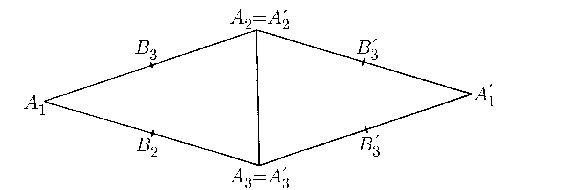
\includegraphics[width=0.56\textwidth]{figures/chapter01-figure03.png}
\caption{两个相邻三角形 ($n=2$)}
\label{fig:ch1-two-adjacent-triangles}
\end{figure}

\MBSourceStatementNumber{lemma}{15}
\begin{Lemma}
\label{lem:ch1-nc-wh-basis}
$W_h$ 中的函数 $w_{hB}e_i$, $B\in U_h$, $1\leq i\leq n$, 构成 $W_h$ 的一组基. 因而 $W_h$ 的维数为 $nN(h)$, 其中 $N(h)$ 是 $U_h$ 中点的数目.
\end{Lemma}

\begin{Proof}
显然这些函数线性无关且张成整个空间 $W_h$: 由命题 \ref{prop:ch1-linear-barycentric-interpolation}, 任意 $u_h\in W_h$ 可写为
\begin{equation}
u_h=\sum_{B\in U_h}u_h(B)w_{hB}.
\label{eq:ch1-nc-wh-expansion}
\end{equation}
\end{Proof}

空间 $W_h$ 不包含于 $H_0^1(\Omega)$. 事实上, 对某个 $u_h\in W_h$, 导数 $D_iu_h$ 是位于各单纯形面上的 Dirac 分布与一个阶梯函数 $D_{ih}u_h$ 之和, 后者几乎处处定义为
\begin{equation}
D_{ih}u_h(x)=D_iu_h(x),
\qquad\forall x\in S,
\quad\forall S\in T_h.
\label{eq:ch1-nc-broken-derivative}
\end{equation}
因为 $u_h$ 在 $S$ 上为线性函数, $D_{ih}u_h$ 在每个单纯形上为常数.

在 $W_h$ 上赋予下述标量积:
\begin{equation}
[[u_h,v_h]]_h=(u_h,v_h)+\sum_{i=1}^n(D_{ih}u_h,D_{ih}v_h),
\label{eq:ch1-nc-wh-full-product}
\end{equation}
它是 $H_0^1(\Omega)$ 标量积的离散类似物:
\begin{equation}
[[u,v]]=(u,v)+\sum_{i=1}^n(D_iu,D_iv).
\label{eq:ch1-nc-h01-full-product}
\end{equation}

\emph{空间 $F$ 与算子 $\omega,p_h$.} 与第 \ref{subsec:ch1-finite-difference-approximation} 节一样, 取 $F=L^2(\Omega)^{n+1}$, 并令 $\omega$ 为同构
\begin{equation}
u\in H_0^1(\Omega)\longmapsto
\omega u=(u,D_1u,\ldots,D_nu)\in F.
\label{eq:ch1-nc-h01-embedding}
\end{equation}
类似地, 定义算子 $p_h$ 为
\begin{equation}
u_h\in W_h\longmapsto
p_hu_h=(\widetilde u_h,\widetilde{D_{1h}u_h},\ldots,
\widetilde{D_{nh}u_h})\in F.
\label{eq:ch1-nc-prolongation}
\end{equation}
与第 \ref{subsec:ch1-finite-difference-approximation} 节一样, $\widetilde g$ 表示在 $\Omega$ 中等于 $g$, 在 $\Omega$ 的补集中等于零的函数. 各算子 $p_h$ 的范数均为 1, 因而稳定.

\emph{算子 $r_h$.} 对 $u\in\mathcal D(\Omega)$, 通过
\begin{equation}
u_h(B)=u(B),
\qquad\forall B\in U_h
\label{eq:ch1-nc-point-restriction}
\end{equation}
定义 $r_hu=u_h$.

\MBSourceStatementNumber{proposition}{12}
\begin{Proposition}
\label{prop:ch1-nc-h01-stable-convergent}
若 $h$ 属于 $\Omega$ 的正则剖分 $\mathcal H_\alpha$, 则上述 $H_0^1(\Omega)$ 的逼近稳定且收敛.
\end{Proposition}

\begin{Proof}
需要验证定义 \ref{def:ch1-convergent-external-approximation} 中的条件 (C1) 和 (C2).

对条件 (C2), 需要证明对每个 $u\in\mathcal D(\Omega)$, 当 $\rho(h)\to0$ 时,
\begin{equation}
u_h\longrightarrow u
\quad\text{在 }L^2(\Omega)\text{ 中},
\label{eq:ch1-nc-l2-convergence}
\end{equation}
\begin{equation}
D_{ih}u_h\longrightarrow D_iu
\quad\text{在 }L^2(\Omega)\text{ 中}.
\label{eq:ch1-nc-derivative-convergence}
\end{equation}
在每个单纯形 $S$ 上, 可对 $u$ 的每个分量应用 \eqref{eq:ch1-general-simplex-interpolation-error}, 得到
\begin{equation}
\begin{aligned}
\sup_{x\in S}|u(x)-u_h(x)|&\leq c\eta_2(u)\rho_S^2,\\
\sup_{x\in S}|D_iu(x)-D_iu_h(x)|
&\leq c\eta_2(u)\frac{\rho_S^2}{\rho'_S}.
\end{aligned}
\label{eq:ch1-nc-local-interpolation-error}
\end{equation}
因此
\begin{equation}
\|p_hu_h-\omega u\|_F
\leq c(u)\alpha\rho(h)+[[u]]_{H_0^1(\Omega-\Omega(h))},
\label{eq:ch1-nc-global-interpolation-error}
\end{equation}
而当 $\rho(h)\to0$ 时, 右端趋于零.

为证明条件 (C1), 假设 $p_{h'}u_{h'}$ 在 $F$ 中弱收敛于 $\phi=(\phi_0,\ldots,\phi_n)$. 这意味着
\begin{equation}
u_{h'}\rightharpoonup\phi_0
\quad\text{在 }L^2(\Omega)\text{ 中},
\label{eq:ch1-nc-weak-function}
\end{equation}
\begin{equation}
D_{ih'}u_{h'}\rightharpoonup\phi_i
\quad\text{在 }L^2(\Omega)\text{ 中},
\qquad1\leq i\leq n.
\label{eq:ch1-nc-weak-derivatives}
\end{equation}
因为这些函数具有包含于 $\Omega$ 的紧支集, \eqref{eq:ch1-nc-weak-function} 和 \eqref{eq:ch1-nc-weak-derivatives} 等价于
\begin{equation}
\widetilde u_{h'}\rightharpoonup\widetilde\phi_0
\quad\text{在 }L^2(\mathbb R^n)\text{ 中},
\label{eq:ch1-nc-extended-weak-function}
\end{equation}
\begin{equation}
\widetilde{D_{ih'}u_{h'}}\rightharpoonup\widetilde\phi_i
\quad\text{在 }L^2(\mathbb R^n)\text{ 中},
\qquad1\leq i\leq n.
\label{eq:ch1-nc-extended-weak-derivatives}
\end{equation}
其中 $\widetilde g$ 在 $\Omega$ 中等于 $g$, 在 $\mathbb R^n-\Omega$ 中等于零. 若能证明
\begin{equation}
\widetilde\phi_i=D_i\widetilde\phi_0,
\qquad1\leq i\leq n,
\label{eq:ch1-nc-identify-weak-derivative}
\end{equation}
则 $\widetilde\phi_0\in H^1(\mathbb R^n)$, 从而 $\phi_0\in H_0^1(\Omega)$ 且 $\phi_i=D_i\phi_0$. 这正是说 $\phi=\omega u$, $u=\phi_0$.

设 $\theta$ 是 $\mathcal D(\mathbb R^n)$ 中任意检验函数. 则
\[
\int_{\mathbb R^n}\widetilde u_{h'}D_i\theta\,dx
\longrightarrow\int_{\mathbb R^n}\phi_0D_i\theta\,dx,
\]
\[
\int_{\mathbb R^n}\widetilde{D_{ih'}u_{h'}}\theta\,dx
\longrightarrow\int_{\mathbb R^n}\phi_i\theta\,dx.
\]
如果证明对每个 $\theta\in\mathcal D(\mathbb R^n)$,
\[
\int_{\mathbb R^n}\phi_i\theta\,dx
=-\int_{\mathbb R^n}\phi_0D_i\theta\,dx,
\]
即
\[
J_{h'}^i=\int_{\mathbb R^n}\widetilde u_{h'}D_i\theta\,dx
+\int_{\mathbb R^n}\widetilde{D_{ih'}u_{h'}}\theta\,dx
\longrightarrow0
\]
当 $\rho(h')\to0$, 则 \eqref{eq:ch1-nc-identify-weak-derivative} 成立. 根据第 \ref{subsubsec:ch1-nc-auxiliary-estimates} 节证明的技术估计 \eqref{eq:ch1-nc-jh-h1-estimate},
\begin{equation}
|J_h^i|\leq c(n,\Omega)\alpha\rho(h)
\|\theta\|_{H^1(\Omega)}\|u_h\|_h,
\label{eq:ch1-nc-jh-weak-estimate}
\end{equation}
显然当 $\rho(h)\to0$ 时, $J_h^i\to0$.
\end{Proof}

\emph{离散 Poincaré 不等式.} 下面的离散 Poincaré 不等式使我们能够在上述空间 $W_h$ 上赋予另一个标量积 $((\cdot,\cdot))_h$, 它是 $H_0^1(\Omega)$ 的标量积 $((\cdot,\cdot))$ 的离散类似物, 见 \eqref{eq:ch1-h01-gradient-inner-product} 和命题 \ref{prop:ch1-h01-gradient-inner-product}.

\MBSourceStatementNumber{proposition}{13}
\begin{Proposition}
\label{prop:ch1-nc-discrete-poincare}
设 $\Omega$ 是 $\mathbb R^n$ 中的有界集. 则存在仅依赖于 $\Omega$ 与 \eqref{eq:ch1-regular-triangulation-shape-bound} 中常数 $\alpha$ 的常数 $c(\Omega,\alpha)$, 使得
\begin{equation}
|u_h|_{L^2(\Omega)}^2
\leq c(\Omega,\alpha)\sum_{i=1}^n|D_{ih}u_h|_{L^2(\Omega)}^2
\label{eq:ch1-nc-discrete-poincare-scalar}
\end{equation}
对任意如下形式的标量函数成立:
\begin{equation}
u_h=\sum_{B\in U_h}u_h(B)w_{hB}.
\label{eq:ch1-nc-scalar-expansion-repeat}
\end{equation}
对 \eqref{eq:ch1-nc-wh-expansion} 形式的向量函数也有类似不等式:
\begin{equation}
|u_h|_{L^2(\Omega)}\leq c'(\Omega,\alpha)\|u_h\|_h,
\qquad\forall u_h\in W_h,
\label{eq:ch1-nc-discrete-poincare-vector}
\end{equation}
其中
\begin{equation}
\|u_h\|_h=
\left(\sum_{i=1}^n|D_{ih}u_h|_{L^2(\Omega)}^2\right)^{1/2}.
\label{eq:ch1-nc-broken-gradient-norm}
\end{equation}
\end{Proposition}

\begin{Proof}
不等式 \eqref{eq:ch1-nc-discrete-poincare-vector} 立即由 \eqref{eq:ch1-nc-discrete-poincare-scalar} 得到. 为证明 \eqref{eq:ch1-nc-discrete-poincare-scalar}, 将证明对每个 \eqref{eq:ch1-nc-scalar-expansion-repeat} 形式的 $u_h$ 以及每个 $\theta\in\mathcal D(\Omega)$,
\begin{equation}
\left|\int_\Omega u_h\theta\,dx\right|
\leq c(\Omega,\alpha)|\theta|_{L^2(\Omega)}\|u_h\|_h.
\label{eq:ch1-nc-poincare-duality-bound}
\end{equation}
由于 $\mathcal D(\Omega)$ 在 $L^2(\Omega)$ 中稠密, \eqref{eq:ch1-nc-poincare-duality-bound} 蕴含 \eqref{eq:ch1-nc-discrete-poincare-scalar}.

以 $\chi$ 表示 Dirichlet 问题
\[
\Delta\chi=\theta\quad\text{在 }\Omega\text{ 中},
\qquad\chi\in H_0^1(\Omega)
\]
的解. 函数 $\chi$ 在 $\Omega$ 上为 $C^\infty$, 且
\begin{equation}
\|\chi\|_{H^2(\Omega)}\leq c_0(\Omega)|\theta|_{L^2(\Omega)}.
\label{eq:ch1-nc-dirichlet-h2-estimate}
\end{equation}
严格说来, 只有当 $\Omega$ 足够光滑时该不等式才成立. 在一般情形下, 若通过 $\Delta\chi=\theta$, $\chi\in H_0^1(\Omega')$ 定义 $\chi$, 其中 $\Omega'$ 光滑且 $\Omega'\supset\Omega$, 则 \eqref{eq:ch1-nc-dirichlet-h2-estimate} 成立. 这不影响下文.

于是
\[
\int_\Omega u_h\theta\,dx
=\sum_{S\in T_h}\int_Su_h\Delta\chi\,dx.
\]
在每个 $S$ 上应用 Green 公式得到
\[
\int_Su_h\Delta\chi\,dx
=\int_{\partial S}u_h\frac{\partial\chi}{\partial\nu}\,d\Gamma
-\int_S\operatorname{grad}u_h\cdot\operatorname{grad}\chi\,dx.
\]
因而
\begin{equation}
\begin{aligned}
\left|\int_\Omega u_h\theta\,dx\right|
&\leq|((u_h,\chi))_h|+|J_h|\\
&\leq\|u_h\|_h\|\chi\|_{H^1(\Omega)}+|J_h|\\
&\leq c(\Omega)|\theta|_{L^2(\Omega)}\|u_h\|_h+|J_h|,
\end{aligned}
\label{eq:ch1-nc-duality-green-bound}
\end{equation}
其中
\[
|J_h|=\left|\sum_{S\in T_h}\int_{\partial S}
u_h\frac{\partial\chi}{\partial\nu}\,d\Gamma\right|.
\]
显然
\begin{equation}
J_h=\sum_{i=1}^nJ_h^i,
\label{eq:ch1-nc-jh-component-sum}
\end{equation}
其中
\[
J_h^i=\sum_{S\in T_h}\int_{\partial S}u_h\chi_i\nu_i\,d\Gamma,
\]
并且
\begin{equation}
\chi_i=\frac{\partial\chi}{\partial x_i}.
\label{eq:ch1-nc-chi-component}
\end{equation}
这里 $\nu_1,\ldots,\nu_n$ 是 $\partial S$ 的单位法向量 $\nu$ 的各分量. 由 Green 公式,
\[
\int_{\partial S}u_h\chi_i\nu_i\,d\Gamma
=\int_S\frac{\partial}{\partial x_i}(u_h\chi_i)\,dx,
\]
所以
\[
J_h^i=\int_\Omega\frac{\partial}{\partial x_i}(u_h\chi_i)\,dx.
\]
在命题 \ref{prop:ch1-nc-h01-stable-convergent} 的证明中已经考虑过这一表达式. 使用估计 \eqref{eq:ch1-nc-jh-weak-estimate} 得到
\[
|J_h^i|\leq c(n,\Omega)\alpha\rho(h)
\|\chi_i\|_{H^1(\Omega)}\|u_h\|_h,
\]
\[
|J_h^i|\leq c(n,\Omega)\alpha\rho(h)
\|\chi_i\|_{H^2(\Omega)}\|u_h\|_h.
\]
由 \eqref{eq:ch1-nc-dirichlet-h2-estimate} 和 \eqref{eq:ch1-nc-jh-component-sum},
\begin{equation}
|J_h|\leq c(n,\Omega)\alpha\rho(h)
|\theta|_{L^2(\Omega)}\|u_h\|_h.
\label{eq:ch1-nc-jh-duality-estimate}
\end{equation}
结合 \eqref{eq:ch1-nc-duality-green-bound} 与 \eqref{eq:ch1-nc-jh-duality-estimate}, 恰好得到 \eqref{eq:ch1-nc-poincare-duality-bound}, 其中
\[
c(\Omega,\alpha)=c(\Omega)+c(n,\Omega)\alpha\rho(h).
\]
这里 $\rho(h)$ 显然有界, 例如 $\rho(h)\leq\operatorname{diameter}\Omega$.
\end{Proof}

\MBSourceStatementNumber{proposition}{14}
\begin{Proposition}
\label{prop:ch1-nc-h01-gradient-product}
设 $\Omega$ 是有界 Lipschitz 集. 若在空间 $W_h$ 上赋予标量积
\begin{equation}
((u_h,v_h))_h=\sum_{i=1}^n(D_{ih}u_h,D_{ih}v_h),
\label{eq:ch1-nc-wh-gradient-product}
\end{equation}
并保持命题 \ref{prop:ch1-nc-h01-stable-convergent} 的其他部分不变, 则这个 $H_0^1(\Omega)$ 的逼近仍然稳定且收敛.
\end{Proposition}

\begin{Proof}
本命题与命题 \ref{prop:ch1-nc-h01-stable-convergent} 的唯一区别来自算子 $p_h$ 的稳定性. 命题 \ref{prop:ch1-nc-discrete-poincare} 与 \eqref{eq:ch1-nc-discrete-poincare-vector} 完全克服了这一困难, 它们给出
\begin{equation}
\|u_h\|_h\leq[[u_h]]_h\leq c(\Omega)\|u_h\|_h,
\qquad\forall u_h\in W_h.
\label{eq:ch1-nc-equivalent-discrete-norms}
\end{equation}
\end{Proof}

\subsubsection{空间 \texorpdfstring{$V$}{V} 的逼近 (APX5)}
\label{subsubsec:ch1-apx5-v-approximation}

设 $\Omega$ 是 $\mathbb R^n$ 中有界 Lipschitz 集, $\mathcal V$ 是通常的空间 \eqref{eq:ch1-test-divergence-free-space}, $V$ 是它在 $\mathbf H_0^1(\Omega)$ 中的闭包.

现在定义一个与上述 $H_0^1(\Omega)$ 的逼近类似的 $V$ 的逼近. 与此前一样, 取 $F=L^2(\Omega)^{n+1}$, 并令 $\omega\in\mathcal L(V,F)$ 为线性算子
\begin{equation}
u\in V\longmapsto\omega u=\{u,D_1u,\ldots,D_nu\}.
\label{eq:ch1-apx5-v-embedding}
\end{equation}

\emph{空间 $V_h$.} $V_h$ 是上述空间 $W_h$ 的子空间:
\begin{equation}
V_h=\left\{u_h\in W_h,\ \sum_{i=1}^nD_{ih}u_{ih}=0\right\}.
\label{eq:ch1-apx5-vh-definition}
\end{equation}
\eqref{eq:ch1-apx5-vh-definition} 中关于 $u_h$ 散度的条件等价于
\begin{equation}
\operatorname{div}u_h=0
\quad\text{在 }S\text{ 中},
\qquad\forall S\in T_h.
\label{eq:ch1-apx5-elementwise-divergence}
\end{equation}
在空间 $V_h$ 上赋予由 $W_h$ 诱导的标量积 $((u_h,v_h))_h$.

\emph{算子 $p_h$.} 与前面一样,
\[
p_hu_h=\{u_h,D_{1h}u_h,\ldots,D_{nh}u_h\}.
\]
由不等式 \eqref{eq:ch1-nc-discrete-poincare-vector}(或 \eqref{eq:ch1-nc-equivalent-discrete-norms}), 各算子 $p_h$ 稳定.

\emph{算子 $r_h$.} 对 $u\in\mathcal V$, 需要定义 $r_hu=u_h\in V_h$. 因为 $u_h$ 必须满足 \eqref{eq:ch1-apx5-elementwise-divergence}, 用于逼近 $H_0^1(\Omega)$ 的算子 $r_h$ 不能满足全部要求. 改取下述算子 $r_h$: $u_h=r_hu$ 由各值 $u_h(B)$, $B\in U_h$, 刻画. 若 $B\in U_h$ 是某个 $n$-单纯形 $S\in T_h$ 的某个 $(n-1)$-维面 $S'$ 的重心, 则令
\begin{equation}
u_h(B)=\frac1{\operatorname{meas}_{n-1}(S')}
\int_{S'}u\,d\Gamma.
\label{eq:ch1-apx5-face-average-restriction}
\end{equation}
下面说明 $u_h\in V_h$. 因为 $\operatorname{div}u_h$ 在每个单纯形 $S$ 上为常数, 条件 \eqref{eq:ch1-apx5-elementwise-divergence} 等价于
\[
\int_S\operatorname{div}u_h\,dx=0,
\qquad\forall S\in T_h.
\]
应用 Green 公式得到
\[
\int_S\operatorname{div}u_h\,dx
=\sum_{S'\in\partial^+S}\int_{S'}u_h\cdot\nu_{S'}\,d\Gamma,
\]
其中 $\partial^+S$ 是 $S$ 的 $(n-1)$-维面集合. 由 \eqref{eq:ch1-apx5-face-average-restriction}, 上式等于
\[
\sum_{S'\in\partial^+S}\int_{S'}u\cdot\nu_{S'}\,d\Gamma
=\int_{\partial S}u\cdot\nu\,d\Gamma
=\int_S\operatorname{div}u\,dx,
\]
而最后一个积分因 $\operatorname{div}u=0$ 而为零.

\MBSourceStatementNumber{proposition}{15}
\begin{Proposition}
\label{prop:ch1-apx5-v-stable-convergent}
若 $h$ 属于 $\Omega$ 的正则剖分 $\mathcal H_\alpha$, 则上述 $V$ 的外逼近稳定且收敛.
\end{Proposition}

\begin{Proof}
已经指出各 $p_h$ 稳定. 先验证定义 \ref{def:ch1-convergent-external-approximation} 的条件 (C2). 假设
\begin{equation}
p_{h'}u_{h'}\rightharpoonup\phi
\quad\text{在 }F\text{ 中}.
\label{eq:ch1-apx5-weak-limit}
\end{equation}
与命题 \ref{prop:ch1-nc-h01-stable-convergent} 中完全一样, 可得
\begin{equation}
\phi=\omega u,
\qquad u\in\mathbf H_0^1(\Omega).
\label{eq:ch1-apx5-limit-h01}
\end{equation}
这里还必须证明 $u\in V$, 即 $\operatorname{div}u=0$. 而 \eqref{eq:ch1-apx5-weak-limit} 特别意味着
\[
\sum_{i=1}^nD_{ih'}u_{ih'}
ightharpoonup\operatorname{div}u
\quad\text{在 }L^2(\Omega)\text{ 中}.
\]
由于 $\sum_{i=1}^nD_{ih'}u_{ih'}$ 恒等于零, $\operatorname{div}u=0$.

再验证条件 (C1). 若 $u\in\mathcal V$, 以 $u_h$ 表示 $r_hu$, 并令 $v_h$ 为 $W_h$ 中满足
\[
v_h(B)=u(B),
\qquad\forall B\in U_h
\]
的函数. 命题 \ref{prop:ch1-nc-h01-stable-convergent} 中已证明
\begin{equation}
\|p_hv_h-\omega u\|_F
\leq c(u)\alpha\rho(h)+[[u]]_{H^1(\Omega-\Omega(h))}.
\label{eq:ch1-apx5-point-interpolant-error}
\end{equation}
现在只需证明当 $\rho(h)\to0$ 时,
\begin{equation}
\|p_hu_h-p_hv_h\|_F=[[u_h-v_h]]_h\longrightarrow0.
\label{eq:ch1-apx5-interpolants-difference}
\end{equation}
由 \eqref{eq:ch1-nc-equivalent-discrete-norms}, 只需证明当 $\rho(h)\to0$ 时 $\|u_h-v_h\|_h\to0$.

$U_h$ 中每个 $B$ 都是某个单纯形 $S$ 的某个面 $S'$ 的重心. 可写成
\begin{equation}
u(x)=u(B)+\sum_{i=1}^n\frac{\partial u}{\partial x_i}(B)(x_i-\beta_i)+\sigma(x),
\label{eq:ch1-apx5-taylor-face-barycenter}
\end{equation}
其中 $(\beta_1,\ldots,\beta_n)$ 是 $B$ 的坐标, 并且
\begin{equation}
|\sigma(x)|\leq c(u)\rho'_S,
\qquad\forall x\in S.
\label{eq:ch1-apx5-taylor-remainder}
\end{equation}
在 $S'$ 上对 \eqref{eq:ch1-apx5-taylor-face-barycenter} 积分, 由 $\int_{S'}(x_i-\beta_i)\,dx=0$ 得
\[
u_h(B)=v_h(B)
+\left(\int_{S'}\sigma(x)\,dx\right)
\left(\int_{S'}dx\right)^{-1}.
\]
由 \eqref{eq:ch1-apx5-taylor-remainder},
\begin{equation}
u_h(B)-v_h(B)=\epsilon_h(B),
\label{eq:ch1-apx5-nodal-error}
\end{equation}
且
\begin{equation}
|\epsilon_h(B)|\leq c(u)\rho_S^2.
\label{eq:ch1-apx5-nodal-error-bound}
\end{equation}

在面为 $S_1,\ldots,S_{n+1}$ 的单纯形 $S$ 内,
\[
u_h(x)-v_h(x)=\sum_{i=1}^{n+1}\epsilon_h(B_i)\mu_i(x),
\]
其中 $\mu_1,\ldots,\mu_{n+1}$ 是 $x$ 关于 $B_1,\ldots,B_{n+1}$ 的重心坐标. 因而在 $S$ 中,
\[
|\operatorname{grad}(u_h-v_h)|
\leq c(u)\rho_S^2\sum_{i=1}^{n+1}|\operatorname{grad}\mu_i|.
\]
由引理 \ref{lem:ch1-barycentric-gradient-bound} 和 \eqref{eq:ch1-regular-triangulation-shape-bound},
\[
|\operatorname{grad}(u_h-v_h)|
\leq c(u)\frac{\rho_S^2}{\rho'_S}.
\]
因此在整个 $\Omega$ 中,
\begin{equation}
|D_{ih}(u_h-v_h)(x)|\leq c(u)\alpha\rho(h),
\label{eq:ch1-apx5-broken-derivative-error}
\end{equation}
从而
\begin{equation}
\|u_h-v_h\|_h\leq c(u,\alpha,\Omega)\rho(h),
\label{eq:ch1-apx5-broken-norm-error}
\end{equation}
并且
\begin{equation}
\|p_hu_h-\omega u\|_F
\leq c(u)\alpha\rho(h)+[[u]]_{H^1(\Omega-\Omega(h))}.
\label{eq:ch1-apx5-global-convergence-estimate}
\end{equation}
\end{Proof}

\subsubsection{Stokes 问题的逼近}
\label{subsubsec:ch1-apx5-stokes}

使用上述 $V$ 的逼近及第 \ref{subsec:ch1-general-convergence-theorem} 节的一般结果, 可为 Stokes 问题提出另一种格式.

设 $f\in\mathbf L^2(\Omega)$ 且 $\nu>0$. 使用上述记号, 令
\begin{equation}
a_h(u_h,v_h)=\nu((u_hv_h))_h,
\qquad\forall u_h,v_h\in V_h,
\label{eq:ch1-apx5-bilinear-form}
\end{equation}
\begin{equation}
\langle\ell_h,v_h\rangle=(f,v_h),
\qquad\forall v_h\in V_h.
\label{eq:ch1-apx5-linear-form}
\end{equation}
近似问题为
\begin{equation}
\left\{
\begin{array}{l}
\text{求 }u_h\in V_h\text{ 使得}\\
\nu((u_h,v_h))_h=(f,v_h),
\qquad\forall v_h\in V_h.
\end{array}
\right.
\label{eq:ch1-apx5-stokes-problem}
\end{equation}
问题 \eqref{eq:ch1-apx5-stokes-problem} 的解 $u_h$ 存在且唯一. 若 $\rho(h)\to0$, 且 $h$ 属于正则剖分 $\mathcal H_\alpha$, 则
\begin{equation}
\begin{aligned}
u_h&\longrightarrow u
&&\text{在 }\mathbf L^2(\Omega)\text{ 中强收敛},\\
D_{ih}u_h&\longrightarrow D_iu
&&\text{在 }\mathbf L^2(\Omega)\text{ 中强收敛},
\quad1\leq i\leq n.
\end{aligned}
\label{eq:ch1-apx5-stokes-convergence}
\end{equation}
这当然来自定理 \ref{thm:ch1-general-approximation-convergence}.

像第 \ref{subsec:ch1-finite-difference-approximation} 节以及其他逼近一样, 可以引入离散压力. 它是下述类型的阶梯函数 $\pi_h$:
\begin{equation}
\pi_h=\sum_{S\in T_h}\pi_h(S)\chi_{hS},
\label{eq:ch1-apx5-discrete-pressure}
\end{equation}
其中 $\pi_h(S)$ 是 $\pi_h$ 在 $S$ 上的值, $\pi_h(S)\in\mathbb R$, $\chi_{hS}$ 是 $S$ 的示性函数. 函数 $\pi_h$ 满足
\begin{equation}
\nu((u_h,v_h))_h-(\pi_h,\operatorname{div}_hv_h)
=(f,v_h),
\qquad\forall v_h\in W_h,
\label{eq:ch1-apx5-velocity-pressure-system}
\end{equation}
其中
\begin{equation}
\operatorname{div}_hv_h=\sum_{i=1}^nD_{ih}v_{ih}.
\label{eq:ch1-apx5-discrete-divergence}
\end{equation}

分别作为 \eqref{eq:ch1-stokes-variational-problem} 与 \eqref{eq:ch1-apx5-velocity-pressure-system} 的解, $u$ 与 $u_h$ 之间的误差可像第 \ref{subsec:ch1-finite-difference-approximation} 节那样估计. 假设 $\Omega$ 有多边形边界, $\Omega(h)=\Omega$, 且 $u\in C^3(\overline\Omega)$, $p\in C^1(\overline\Omega)$. 可用与 \eqref{eq:ch1-apx5-face-average-restriction} 类似的公式定义逼近 $r_hu$, 并且不难看出估计 \eqref{eq:ch1-apx5-global-convergence-estimate} 仍成立:
\begin{equation}
\|p_hr_hu-\omega u\|_F\leq c(u,\alpha)\rho(h).
\label{eq:ch1-apx5-smooth-interpolation-error}
\end{equation}

下面的引理稍后证明.

\MBSourceStatementNumber{lemma}{16}
\begin{Lemma}
\label{lem:ch1-apx5-consistency}
设 $u,p$ 表示 \eqref{eq:ch1-stokes-variational-problem}–\eqref{eq:ch1-stokes-weak-incompressibility} 的精确解, 并假设 $u\in C^3(\overline\Omega)$. 则
\begin{equation}
a_h(u,v_h)=(f,v_h)+\ell_h(v_h),
\qquad\forall v_h\in V_h,
\label{eq:ch1-apx5-consistency-identity}
\end{equation}
其中
\begin{equation}
|\ell_h(v_h)|\leq c(u,p)\rho(h)\|v_h\|_h.
\label{eq:ch1-apx5-consistency-bound}
\end{equation}
\end{Lemma}

暂时接受此引理, 可见
\[
a_h(u_h-u,v_h)=-\ell_h(v_h),
\qquad\forall v_h\in V_h,
\]
\[
a_h(u_h-r_hu,v_h)=a_h(u-r_hu,v_h)-\ell_h(v_h).
\]
取 $v_h=u_h-r_hu$ 并使用 \eqref{eq:ch1-apx5-linear-form}, 得到
\[
\nu\|u_h-r_hu\|_h^2
\leq\nu\|u-r_hu\|_h\|u_h-r_hu\|_h
+|\ell_h(u_h-r_hu)|.
\]
于是估计 \eqref{eq:ch1-apx5-smooth-interpolation-error} 与 \eqref{eq:ch1-apx5-consistency-bound} 给出
\begin{equation}
\nu\|u_h-r_hu\|_H\leq c(u,p,\alpha,\Omega)\rho(h).
\label{eq:ch1-apx5-stokes-error}
\end{equation}
更确切地说, \eqref{eq:ch1-apx5-stokes-error} 中的常数 $c$ 只依赖于 $u$ 在 $C^3(\overline\Omega)$ 中的范数和 $p$ 在 $C^1(\overline\Omega)$ 中的范数.

\begin{Proof}[引理 \ref{lem:ch1-apx5-consistency} 的证明]
在 $L^2(\Omega)$ 中取方程
\begin{equation}
-\nu\Delta u+\operatorname{grad}p=f
\label{eq:ch1-apx5-strong-momentum}
\end{equation}
与 $v_h$ 的标量积. 因为 $\Omega=\Omega(h)$, 得到
\begin{equation}
\sum_{S\in T_h}\{-\nu(\Delta u,v_h)_S
+(\operatorname{grad}p,v_h)_S-(f,v_h)_S\}=0.
\label{eq:ch1-apx5-elementwise-momentum}
\end{equation}
在每个单纯形 $S$ 上应用 Green 公式得到
\[
\sum_{S\in T_h}\{-\nu(\Delta u,v_h)_S
+(\operatorname{grad}p,v_h)_S-(f,v_h)_S\}
=a_h(u,v_h)-(f,v_h)-\ell_h(v_h)=0,
\]
其中
\[
\ell_h(v_h)=\sum_{S\in T_h}\int_{\partial S}
\left(\nu\frac{\partial u}{\partial\vec\nu}v_h
-pv_h\vec\nu\right)d\Gamma.
\]
这里用 $\vec\nu$ 表示 $\partial S$ 的单位法向量, 以免与常数 $\nu>0$ 混淆. 对 $\ell_h$ 的估计 \eqref{eq:ch1-apx5-consistency-bound} 完全按照引理 \ref{lem:ch1-nc-boundary-cancellation}, \ref{lem:ch1-nc-boundary-difference} 和 \ref{lem:ch1-nc-boundary-cauchy} 的方法证明, 见第 \ref{subsubsec:ch1-nc-auxiliary-estimates} 节.
\end{Proof}

\MBSourceStatementNumber{remark}{9}
\begin{Remark}
\label{rem:ch1-apx5-basis-and-uses}
二维情形下存在 $V_h$ 的一组简单基, 见 Crouzeix [1].

次数 $k>1$ 的非协调分片多项式有限元也已用于逼近 $H_0^1(\Omega)$ 或空间 $V$.

M. Fortin [2] 指出, 空间 $V$ 不能由一次协调有限元(即分片线性函数)逼近. 因而本节研究的逼近对 Stokes 与 Navier--Stokes 问题无疑非常有用.

F. Thomasset [2] 已使用这些单元对黏性不可压缩流进行了若干计算.
\end{Remark}

\subsubsection{辅助估计}
\label{subsubsec:ch1-nc-auxiliary-estimates}

这里证明前面用过且在 \MBUnresolvedReference{chapter}{Chapter 2} 中也会用到的一些辅助技术估计. 这些估计涉及表达式
\begin{equation}
J_h^i=\int_\Omega\frac{\partial}{\partial x_i}(u_h\phi)\,dx,
\label{eq:ch1-nc-auxiliary-jh}
\end{equation}
其中 $u_h\in W_h$, $i=1,\ldots,n$, 而 $\phi$ 取不同类型的函数.

下面的证明是直接的. 使用有限元的一般结果可以简化它们.

\MBSourceStatementNumber{proposition}{16}
\begin{Proposition}
\label{prop:ch1-nc-jh-h1-estimate}
若 $\phi\in H^1(\Omega)$ 且 $u_h\in W_h$, 则
\begin{equation}
|J_h^i|\leq c(n,\Omega)\alpha\rho(h)
\|\phi\|_{H^1(\Omega)}\|u_h\|_h.
\label{eq:ch1-nc-jh-h1-estimate}
\end{equation}
\end{Proposition}

证明由下面几个引理给出.

\MBSourceStatementNumber{lemma}{17}
\begin{Lemma}
\label{lem:ch1-nc-boundary-cancellation}
有
\begin{equation}
J_h^i=\sum_{S\in T_h}\sum_{S'\in\partial^+S}
\int_{S'}u_h\phi\nu_{i,S'}\,d\Gamma,
\label{eq:ch1-nc-jh-face-sum}
\end{equation}
其中 $\partial^+S$ 是 $S$ 的 $(n-1)$-维面集合, $\nu_{i,S'}$ 是单位向量 $\nu_{S'}$ 的第 $i$ 个分量, $\nu_{S'}$ 与 $S'$ 正交并相对于 $S$ 指向外侧.
\end{Lemma}

\begin{Proof}
因为各函数在 $\Omega(h)$ 外为零,
\[
\begin{aligned}
J_h^i
&=\int_{\Omega(h)}[u_h(D_i\phi)+(D_{ih}u_h)\phi],dx\\
&=\sum_{S\in T_h}\int_S[u_h(D_i\phi)+(D_iu_h)\phi],dx\\
&=\sum_{S\in T_h}\int_SD_i(u_h\phi)\,dx.
\end{aligned}
\]
Green--Stokes 公式给出
\[
\int_SD_i(u_h\phi)\,dx
=\sum_{S'\in\partial^+S}\int_{S'}u_h\phi\nu_{i,S'}\,d\Gamma.
\]
\end{Proof}

原书在此注明, 这样的面有 $n-1$ 个.

\MBSourceStatementNumber{lemma}{18}
\begin{Lemma}
\label{lem:ch1-nc-boundary-difference}
使用引理 \ref{lem:ch1-nc-boundary-cancellation} 的记号,
\begin{equation}
J_h^i=\sum_{S\in T_h}\sum_{S'\in\partial^+S}
\int_{S'}(u_h(x)-u_h(B))(\phi(x)-\phi(S'))
\nu_{i,S'}\,d\Gamma,
\label{eq:ch1-nc-jh-difference-form}
\end{equation}
其中 $B=B_{S'}$ 是 $S'$ 的重心, $\phi(S')$ 是 $\phi$ 在 $S'$ 上的平均值.
\end{Lemma}

\begin{Proof}
先证明
\begin{equation}
J_h^i=\sum_{S\in T_h}\sum_{S'\in\partial^+S}
\int_{S'}(u_h(x)-u_h(B))\phi(x)\nu_{i,S'}\,d\Gamma.
\label{eq:ch1-nc-jh-subtract-barycenter}
\end{equation}
为此只需证明
\begin{equation}
\sum_{S\in T_h}\sum_{S'\in\partial^+S}
\int_{S'}u_h(B)\phi(x)\nu_{i,S'}\,d\Gamma=0.
\label{eq:ch1-nc-jh-barycenter-cancellation}
\end{equation}
若面 $S'$ 属于 $\Omega(h)$ 的边界, 则 $u_h(B)=0$, 该面对和的贡献为零. 若 $S'$ 属于两个相邻单纯形的边界, 则该面对和给出两个符号相反的项: 两项中的 $u_h(B)$ 和 $\phi(x)$ 相同, 而从两个单纯形边界看待 $S'$ 时, $\nu_{i,S'}$ 大小相同、符号相反. 因而 \eqref{eq:ch1-nc-jh-barycenter-cancellation} 中的和为零.

若证明
\begin{equation}
\sum_{S\in T_h}\sum_{S'\in\partial^+S}
\int_{S'}(u_h(x)-u_h(B))\phi(S')\nu_{i,S'}\,d\Gamma=0,
\label{eq:ch1-nc-jh-average-cancellation}
\end{equation}
则容易由 \eqref{eq:ch1-nc-jh-subtract-barycenter} 推出 \eqref{eq:ch1-nc-jh-difference-form}. 而为证明 \eqref{eq:ch1-nc-jh-average-cancellation}, 只需注意
\[
\int_{S'}[u_h(x)-u_h(B)]\phi(S')\nu_{i,S'}\,d\Gamma=0,
\]
因为 $\phi(S')$ 与 $\nu_{i,S'}$ 在 $S'$ 上为常数, 并且
\begin{equation}
\int_{S'}u_h(x)\,d\Gamma
=u_h(B)\int_{S'}d\Gamma,
\label{eq:ch1-nc-linear-face-average}
\end{equation}
这是因为 $u_h$ 在 $S'$ 上为线性函数, 且 $B$ 是 $S'$ 的重心.
\end{Proof}

\MBSourceStatementNumber{lemma}{19}
\begin{Lemma}
\label{lem:ch1-nc-boundary-cauchy}
有
\begin{equation}
|J_h^i|\leq c(n)\sqrt{\alpha\rho(h)}\,\|u_h\|_h
\left(\sum_{S\in T_h}\sum_{S'\in\partial^+S}
\int_{S'}(\phi(x)-\phi(S'))^2\,d\Gamma\right)^{1/2}.
\label{eq:ch1-nc-jh-cauchy-bound}
\end{equation}
\end{Lemma}

\begin{Proof}
因为 $u_h(x)-u_h(B)$ 是 $S'$ 上在 $x=B$ 处为零的线性函数, 可在 $S$ 上写成
\[
u_h(x)-u_h(B)=\sum_{i=1}^n\frac{\partial u_h}{\partial x_i}(x_i-\beta_i),
\]
其中 $\beta_1,\ldots,\beta_n$ 是 $B$ 的坐标. 因而
\[
|u_h(x)-u_h(B)|\leq\rho_S|\operatorname{grad}u_h|,
\qquad\forall x\in S,
\]
并且
\[
\begin{aligned}
&\left|\int_{S'}(u_h(x)-u_h(B))(\phi(x)-\phi(S'))
\nu_{i,S'}\,d\Gamma\right|\\
&\quad\leq\rho_S
\left(\int_{S'}|\operatorname{grad}u_h|^2\,d\Gamma\right)^{1/2}
\left(\int_{S'}(\phi(x)-\phi(S'))^2\,d\Gamma\right)^{1/2}.
\end{aligned}
\]
因为 $\operatorname{grad}u_h$ 在 $S'$ 上为常数,
\[
\int_{S'}(\operatorname{grad}u_h)^2\,d\Gamma
=\operatorname{meas}_{n-1}(S')|\operatorname{grad}u_h|^2.
\]
令 $\xi$ 表示 $S'$ 与 $S$ 的对顶点之间的距离. 熟知
\[
\operatorname{meas}_n(S)=\frac1n\xi\operatorname{meas}_{n-1}(S').
\]
因而
\begin{equation}
\operatorname{meas}_{n-1}(S')
=\frac n\xi\operatorname{meas}_n(S)
\leq\frac n{\rho'_S}\operatorname{meas}_n(S),
\label{eq:ch1-nc-face-measure-bound}
\end{equation}
因为
\begin{equation}
\rho'_S\leq\xi.
\label{eq:ch1-nc-inradius-height-bound}
\end{equation}
式 \eqref{eq:ch1-nc-inradius-height-bound} 成立是因为 $S$ 中最大内接球的直径等于 $\rho'_S$, 且该球包含于由含 $S'$ 的超平面和含对顶点的平行超平面围成的区域中.

因此
\[
\int_{S'}(\operatorname{grad}u_h)^2\,d\Gamma
\leq\frac n{\rho'_S}\int_S|\operatorname{grad}u_h|^2\,dx,
\]
并且
\begin{equation}
\begin{aligned}
|J_h^i|\leq c(n)\sum_{S\in T_h}\sum_{S'\in\partial^+S}
\frac{\rho_S}{\sqrt{\rho'_S}}
&\left(\int_S|\operatorname{grad}u_h|^2\,dx\right)^{1/2}\\
{}\times&\left(\int_{S'}|\phi(x)-\phi(S')|^2\,d\Gamma\right)^{1/2}.
\end{aligned}
\label{eq:ch1-nc-jh-pre-cauchy}
\end{equation}
使用 \eqref{eq:ch1-triangulation-max-diameter}, \eqref{eq:ch1-regular-triangulation-shape-bound} 并对 \eqref{eq:ch1-nc-jh-pre-cauchy} 应用 Schwarz 不等式, 得到 \eqref{eq:ch1-nc-jh-cauchy-bound}.
\end{Proof}

\MBSourceStatementNumber{lemma}{20}
\begin{Lemma}
\label{lem:ch1-nc-uniform-trace}
有
\begin{equation}
\int_{S'}(\phi(x)-\phi(S'))^2\,d\Gamma
\leq c(n)\alpha\rho(h)\int_S(\operatorname{grad}\phi)^2\,dx,
\label{eq:ch1-nc-local-trace-poincare}
\end{equation}
\begin{equation}
\sum_{S\in T_h}\sum_{S'\in\partial^+S}
\int_{S'}(\phi(x)-\phi(S'))^2\,d\Gamma
\leq c(n)\alpha\rho(h)\int_\Omega(\operatorname{grad}\phi)^2\,dx.
\label{eq:ch1-nc-global-trace-poincare}
\end{equation}
\end{Lemma}

\begin{Proof}
式 \eqref{eq:ch1-nc-global-trace-poincare} 直接由 \eqref{eq:ch1-nc-local-trace-poincare} 得到.

若把 \eqref{eq:ch1-nc-local-trace-poincare} 右端的常数 $c(n)\alpha\rho(h)$ 换成依赖于特定单纯形 $S$ 的某个常数 $c(S)$, 则 \eqref{eq:ch1-nc-local-trace-poincare} 是 $H^1(S)$ 中迹定理的显然推论. 式 \eqref{eq:ch1-nc-local-trace-poincare} 的意义在于, 它对 $T_h$ 中各单纯形 $S$ 一致成立.

为证明 \eqref{eq:ch1-nc-local-trace-poincare}, 作坐标变换, 把 $S$ 映到一个固定单纯形 $\overline S$, 再在 $\overline S$ 中应用迹定理不等式, 最后回到 $S$.

为简单起见, 假设 $A_1=0$, $S'$ 包含于超平面 $x_n=0$, 且 $S'$ 的顶点为 $A_1,\ldots,A_n$. 参考单纯形 $\overline S$ 的顶点为 $\overline A_1,\ldots,\overline A_{n+1}$, 其中 $\overline A_1=0$, 且 $\overrightarrow{\overline A_1\overline A_{i+1}}=e_i$, $i=1,\ldots,n$. 与 $S'$ 对应的面是顶点为 $\overline A_1,\ldots,\overline A_n$ 的面 $\overline S'$. 令 $\Lambda$ 为 $\mathbb R^n$ 中由
\[
A_i=\Lambda\overline A_i,
\qquad i=2,\ldots,n+1
\]
定义的线性算子, 令 $\Lambda'$ 为 $\mathbb R^{n-1}$ 中由
\[
A_i=\Lambda'\overline A_i,
\qquad i=2,\ldots,n
\]
定义的线性映射. 对 \eqref{eq:ch1-nc-local-trace-poincare} 左端积分作坐标变换得到
\[
\int_{S'}\sigma(x)^2\,d\Gamma_{S'}
=\frac1{|\det\Lambda'|}\int_{\overline S'}\overline\sigma(\overline x)^2\,d\Gamma_{\overline S},
\]
其中
\begin{equation}
\sigma(x)=\phi(x)-\phi(S'),
\label{eq:ch1-nc-trace-sigma}
\end{equation}
且
\begin{equation}
\overline\sigma(\overline x)=\sigma(x),
\qquad\overline x=\Lambda^{-1}x.
\label{eq:ch1-nc-trace-pullback}
\end{equation}
对单纯形 $\overline S$, 迹定理不等式与 Poincaré 不等式给出, 回顾 $\sigma(B)=0$,
\[
\int_{\overline S'}\overline\sigma^2(\overline x)\,d\Gamma
\leq c(\overline S)\sum_{j=1}^n
\int_{\overline S}\left|\frac{\partial\overline\sigma}{\partial\overline x_j}(\overline x)\right|^2d\overline x.
\]

回到 $S$ 与坐标 $x_i$. 写成
\[
\frac{\partial\overline\sigma}{\partial\overline x_j}(\overline x)
=\sum_{k=1}^n(\Lambda^{-1})_{kj}
\frac{\partial\sigma}{\partial x_k}(\Lambda\overline x),
\]
\[
\sum_{j=1}^n\left|\frac{\partial\overline\sigma}{\partial\overline x_j}(\overline x)\right|^2
\leq\|\Lambda^{-1}\|^2\sum_{k=1}^n
\left|\frac{\partial\sigma}{\partial x_k}(\Lambda\overline x)\right|^2.
\]
因而
\[
\begin{aligned}
\int_{\overline S'}\overline\sigma^2(\overline x)\,d\Gamma
&\leq c(\overline S)\|\Lambda^{-1}\|^2
\int_{\overline S}\sum_{k=1}^n
\left|\frac{\partial\sigma}{\partial x_k}(\Lambda\overline x)\right|^2d\overline x\\
&\leq c(\overline S)|\det\Lambda|\|\Lambda^{-1}\|^2
\int_S(\operatorname{grad}\sigma)^2\,dx.
\end{aligned}
\]
得到
\[
\int_{S'}(\phi(x)-\phi(S'))^2\,d\Gamma
\leq c\frac{|\det\Lambda|}{|\det\Lambda'|}
\|\Lambda^{-1}\|^2\int_S(\operatorname{grad}\phi)^2\,dx.
\]
为证明 \eqref{eq:ch1-nc-local-trace-poincare}, 还需证明
\begin{equation}
\frac{|\det\Lambda|}{|\det\Lambda'|}
\|\Lambda^{-1}\|^2\leq c\alpha\rho(h).
\label{eq:ch1-nc-determinant-trace-bound}
\end{equation}
因为
\[
\frac{\det\Lambda}{\det\Lambda'}
=\frac{\det(\Lambda')^{-1}}{\det\Lambda^{-1}}
=\Lambda_{nn},
\]
且 $|\Lambda_{nn}|\leq\|\Lambda\|$, \eqref{eq:ch1-nc-determinant-trace-bound} 的左端不超过
\[
\|\Lambda\|\|\Lambda^{-1}\|^2.
\]
由引理 \ref{lem:ch1-simplex-linear-map-norms}, 此项不超过
\[
\frac{\rho_{\overline S}}{\rho'_S}
\left(\frac{\rho_S}{\rho'_{\overline S}}\right)^2
\leq c(\overline S)\alpha\rho_S
\leq c(\overline S)\alpha\rho(h).
\]
于是得到 \eqref{eq:ch1-nc-determinant-trace-bound}, 引理证明完毕. 这里 $\Lambda_{nn}$ 是 $\Lambda$ 的 $(n,n)$ 元素; 由于坐标轴的选择, $\Lambda_{in}=0$, $1\leq i\leq n-1$.
\end{Proof}

现在估计 \eqref{eq:ch1-nc-jh-h1-estimate} 显然由 \eqref{eq:ch1-nc-jh-cauchy-bound} 和 \eqref{eq:ch1-nc-global-trace-poincare} 得到.

下面用类似方法证明的不等式将在 \MBUnresolvedReference{chapter}{Chapter 2} 中使用.

\MBSourceStatementNumber{proposition}{17}
\begin{Proposition}
\label{prop:ch1-nc-jh-lp-estimate}
若 $\phi\in W^{1,q'}(\Omega)$, $u_h\in W_h$, $1/q'=1-1/q$, 且对 $1<p<n$ 有 $1/q=1/p-1/n$, 则
\begin{equation}
|J_h^i|\leq c(n,p,\Omega)\alpha^2
\left(\sum_{j=1}^n|D_j\phi|_{L^{q'}(\Omega)}\right)
\left(\sum_{j=1}^n|D_{jh}u_h|_{L^p(\Omega)}\right).
\label{eq:ch1-nc-jh-lp-estimate}
\end{equation}
\end{Proposition}

从 $J_h^i$ 的表达式 \eqref{eq:ch1-nc-jh-difference-form} 出发, 将基本沿用引理 \ref{lem:ch1-nc-boundary-cauchy} 和 \ref{lem:ch1-nc-uniform-trace} 的方法. 主要区别在于, 积分的 Schwarz 不等式被具有适当指数的 Hölder 不等式替代.

\MBSourceStatementNumber{lemma}{21}
\begin{Lemma}
\label{lem:ch1-nc-jh-holder-face}
有
\begin{equation}
|J_h^i|\leq\sum_{S\in T_h}\sum_{S'\in\partial^+S}
\rho_S(\operatorname{meas}_{n-1}(S'))^{1/\gamma'}
|\operatorname{grad}_S u_h|
\left(\int_{S'}|\phi(x)-\phi(S')|^\gamma\,d\Gamma\right)^{1/\gamma},
\label{eq:ch1-nc-jh-holder-face}
\end{equation}
其中 $\operatorname{grad}_S u_h$ 表示 $\operatorname{grad}u_h$ 在 $S$ 上的值, $1\leq i\leq n$.
\end{Lemma}

\begin{Proof}
与引理 \ref{lem:ch1-nc-boundary-cauchy} 一样, 在面 $S'$ 上写成
\[
u_h(x)-u_h(B)=\sum_{i=1}^n\frac{\partial u_h}{\partial x_i}(x_i-\beta_i),
\]
因而
\begin{equation}
|u_h(x)-u_h(B)|\leq\rho_S|\operatorname{grad}u_h|,
\qquad\forall x\in S.
\label{eq:ch1-nc-linear-face-pointwise}
\end{equation}
设 $\gamma$ 为稍后指定的实数, $1<\gamma<\infty$, $\gamma'$ 是其共轭指数, $1/\gamma+1/\gamma'=1$. 有
\[
\begin{aligned}
&\left|\int_{S'}(u_h(x)-u_h(B))(\phi(x)-\phi(S'))
\nu_{i,S'}\,d\Gamma\right|\\
&\quad\leq\rho_S|\operatorname{grad}u_h|
\int_{S'}|\phi(x)-\phi(S')|\,d\Gamma\\
&\quad\leq\rho_S(\operatorname{meas}_{n-1}(S'))^{1/\gamma'}
|\operatorname{grad}u_h|
\left(\int_{S'}|\phi(x)-\phi(S')|^\gamma\,d\Gamma\right)^{1/\gamma}.
\end{aligned}
\]
最后一个不等式是 Hölder 不等式. 求和即得 \eqref{eq:ch1-nc-jh-holder-face}.
\end{Proof}

\MBSourceStatementNumber{lemma}{22}
\begin{Lemma}
\label{lem:ch1-nc-trace-holder}
令
\[
\gamma'=\frac{q(n-1)}n,
\qquad\gamma=\frac{\gamma'}{\gamma'-1}.
\]
则对 $1\leq i\leq n$,
\begin{equation}
\left(\int_{S'}|\phi(x)-\phi(S')|^\gamma\,d\Gamma\right)^{1/\gamma}
\leq c(n,p)\frac{(\operatorname{meas}_{n-1}(S'))^{1/\gamma}}
{(\operatorname{meas}_n(S))^{1/q'}}\rho_S
\left(\int_S|\operatorname{grad}\phi_i|^{q'}\,dx\right)^{1/q'}.
\label{eq:ch1-nc-trace-holder}
\end{equation}
\end{Lemma}

\begin{Proof}
完全按照引理 \ref{lem:ch1-nc-uniform-trace} 的方法, 并使用相同记号. 令 $\sigma(x)=\phi(x)-\phi(S')$, 则
\[
\left(\int_{S'}|\sigma(x)|^\gamma\,d\Gamma_{S'}\right)^{1/\gamma}
=|\det\Lambda'|^{-1/\gamma}
\left(\int_{\overline S'}|\overline\sigma(\overline x)|^\gamma
\,d\Gamma_{\overline S'}\right)^{1/\gamma}.
\]
在参考单纯形 $\overline S$ 上应用 Poincaré 不等式和 Sobolev 嵌入定理:
\[
\begin{aligned}
|\overline\sigma|_{L^\gamma(\overline S')}
&\leq c_0(n,p)|\overline\sigma|_{W^{1/q,q'}(\overline S')}\\
&\leq c_1(n,p)|\overline\sigma|_{W^{1,q'}(\overline S)}\\
&\leq c(\overline S)c_2(n,p)
\left(\sum_{j=1}^n\int_{\overline S}
\left|\frac{\partial\overline\sigma}{\partial\overline x_j}(\overline x)\right|^{q'}d\overline x\right)^{1/q'}.
\end{aligned}
\]
第一步是在 $\overline S'\subset\mathbb R^{n-1}$ 上使用 Sobolev 不等式, 第二步使用迹定理, 见 Lions [1], 第三步使用 Poincaré 不等式. 这里各 $c_i(n,p)$ 也依赖于固定的 $\overline S'$.

使用引理 \ref{lem:ch1-nc-uniform-trace} 中给出的上界, 可见
\[
\begin{aligned}
\left(\sum_{j=1}^n\left|\frac{\partial\overline\sigma}{\partial\overline x_j}(\overline x)\right|^{q'}\right)^{1/q'}
&\leq c(q')\left(\sum_{j=1}^n\left|\frac{\partial\overline\sigma}{\partial\overline x_j}(\overline x)\right|^2\right)^{1/2}\\
&\leq c(q')\|\Lambda^{-1}\|
\left(\sum_{j=1}^n\left|\frac{\partial\sigma}{\partial x_j}(\Lambda\overline x)\right|^2\right)^{1/2}\\
&\leq c'(q')\|\Lambda^{-1}\|
\left(\sum_{j=1}^n\left|\frac{\partial\sigma}{\partial x_j}(\Lambda\overline x)\right|^{q'}\right)^{1/q'}.
\end{aligned}
\]
得到
\[
|\overline\sigma|_{L^\gamma(\overline S')}
\leq c(\overline S)c_3(n,p)\|\Lambda^{-1}\|
\left(\sum_{j=1}^n\int_{\overline S}
\left|\frac{\partial\sigma}{\partial x_j}(\Lambda\overline x)\right|^{q'}d\overline x\right)^{1/q},
\]
回到单纯形 $S$,
\[
|\sigma|_{L^\gamma(\overline S')}
\leq c(\overline S)c_3(n,p)|\det\Lambda|^{1/q'}
\|\Lambda^{-1}\|
\left(\sum_{j=1}^n\int_S
\left|\frac{\partial\sigma}{\partial x_j}(x)\right|^{q'}dx\right)^{1/q}.
\]
最后
\[
\left(\int_{S'}|\sigma(x)|^\gamma\,d\Gamma_{S'}\right)^{1/\gamma}
\leq c(\overline S)c_3(n,p)
\frac{|\det\Lambda|^{1/q'}}{|\det\Lambda'|^{1/\gamma}}
\|\Lambda^{-1}\|
\left(\sum_{j=1}^n\int_S
\left|\frac{\partial\phi}{\partial x_j}\right|^{q'}dx\right)^{1/q}.
\]
注意到
\[
\det\Lambda=\frac{\operatorname{meas}_n(\overline S)}{\operatorname{meas}_n(S)},
\qquad
\det\Lambda'=\frac{\operatorname{meas}_{n-1}(\overline S')}
{\operatorname{meas}_{n-1}(S')},
\]
并由引理 \ref{lem:ch1-simplex-linear-map-norms} 有
\[
\|\Lambda^{-1}\|\leq\frac{\rho_S}{\rho'_{\overline S}},
\]
即可完成证明.
\end{Proof}

\MBSourceStatementNumber{lemma}{23}
\begin{Lemma}
\label{lem:ch1-nc-jh-lp-intermediate}
有
\begin{equation}
|J_h^i|\leq c(n,p)d^2
\left(\sum_{j=1}^n|D_{jh}u_h|_{L^p(\Omega)}\right)
\left(\sum_{j=1}^n|D_j\phi|_{L^{q'}(\Omega)}\right).
\label{eq:ch1-nc-jh-lp-intermediate}
\end{equation}
\end{Lemma}

\begin{Proof}
为证明 \eqref{eq:ch1-nc-jh-lp-intermediate}, 结合 \eqref{eq:ch1-nc-jh-holder-face} 与 \eqref{eq:ch1-nc-trace-holder}. 因为 $1/\gamma+1/\gamma'=1$, 得到
\[
\begin{aligned}
|J_h^i|\leq c(n,p,\Omega)\sum_{S\in T_h}
&\rho_S^2(\operatorname{meas}_n(S))^{-1/q'}
\operatorname{meas}_{n-1}(S')\\
&\cdot|\operatorname{grad}_S u_h|
\left(\int_S|\operatorname{grad}\phi_i|^{q'}dx\right)^{1/q'}.
\end{aligned}
\]
由 \eqref{eq:ch1-nc-inradius-height-bound},
\begin{equation}
|J_h^i|\leq c(n,p,\Omega)
\sum_{S\in T_h}\alpha\rho_S
(\operatorname{meas}_n(S))^{1/q}
|\operatorname{grad}u_h|
\left(\int_S|\operatorname{grad}\phi|^{q'}dx\right)^{1/q'},
\label{eq:ch1-nc-jh-measure-sum}
\end{equation}
因为
\[
\operatorname{meas}_{n-1}(S')
\leq\frac n{\rho'_S}\operatorname{meas}_n(S)
\leq\frac{n\alpha}{\rho_S}\operatorname{meas}_n(S).
\]
$S$ 的 $n$-维测度大于直径为 $\rho'_S$ 的 $n$-维球的测度, 因而
\[
(\rho'_S)^n\leq c(n)\operatorname{meas}_n(S),
\]
以及
\[
\rho_S\leq\alpha\rho'_S
\leq c(n)\alpha(\operatorname{meas}_n(S))^{1/n}.
\]
用此上界从 \eqref{eq:ch1-nc-jh-measure-sum} 推出
\[
|J_h^i|\leq c(n,p,\Omega)\alpha^2\sum_{S\in T_h}
(\operatorname{meas}_n(S))^{1/p}|\operatorname{grad}_S u_h|
\left(\int_S|\operatorname{grad}\phi|^{q'}dx\right)^{1/q'}.
\]
对该和应用指数为 $q$ 和 $q'$ 的 Hölder 不等式, 得到
\begin{equation}
\begin{aligned}
|J_h^i|\leq c(n,p,\Omega)\alpha^2
&\left(\sum_{S\in T_h}(\operatorname{meas}_n(S))^{q/p}
|\operatorname{grad}_S u_h|^q\right)^{1/q}\\
&\cdot\left(\int_{\Omega(h)}|\operatorname{grad}\phi|^{q'}dx\right)^{1/q'}.
\end{aligned}
\label{eq:ch1-nc-jh-global-holder}
\end{equation}
现在, 要得到 \eqref{eq:ch1-nc-jh-lp-intermediate}, 只需证明
\begin{equation}
\left(\sum_{S\in T_h}(\operatorname{meas}_n(S))^{q/p}
|\operatorname{grad}_S u_h|^q\right)^{1/q}
\leq
\left(\sum_{S\in T_h}\operatorname{meas}_n(S)
|\operatorname{grad}u_h|^p\right)^{1/p},
\label{eq:ch1-nc-discrete-lp-lq}
\end{equation}
因为该不等式右端等于
\[
\left(\sum_{S\in T_h}\int_S|\operatorname{grad}u_h|^pdx\right)^{1/p},
\]
而它容易被
\[
c(p)\left(\sum_{j=1}^n|D_{jh}u_h|_{L^p(\Omega)}\right)
\]
控制.
\end{Proof}

在记号作适当修改后, 下一个引理将证明 \eqref{eq:ch1-nc-discrete-lp-lq}.

\MBSourceStatementNumber{lemma}{24}
\begin{Lemma}
\label{lem:ch1-finite-sequence-lp-lq}
设 $a_j,z_j$ 是 $N$ 对非负数, $p,n,q$ 如前. 则
\begin{equation}
\left(\sum_{j=1}^Na_j^{q/p}z_j^q\right)^{1/q}
\leq\left(\sum_{j=1}^Na_jz_j^p\right)^{1/p}.
\label{eq:ch1-finite-sequence-lp-lq}
\end{equation}
\end{Lemma}

\begin{Proof}
当 $N=2$ 时, 证明是初等的. 令
\[
a_1z_1^p+a_2z_2^p=\rho,
\qquad
z_1=\left(\frac{\rho-a_2z_2^p}{a_1}\right)^{1/p},
\]
并注意到函数
\[
z_2\longmapsto a_1^{q/p}z_1^q+a_2^{q/p}z_2^q
=a_1^{q/p}\left(\frac{\rho-a_2z_2^p}{a_1}\right)^{q/p}
+a_2^{q/p}z_2^q
\]
在区间 $[0,(\rho/a_2)^{1/p}]$ 上于端点处取得最大值, 该最大值为 $\rho^{q/p}$.

然后对 $N$ 归纳. 假设 \eqref{eq:ch1-finite-sequence-lp-lq} 对 $N-1$ 项成立, 写成
\begin{equation}
\begin{aligned}
\left(\sum_{j=1}^Na_j^{q/p}z_j^q\right)^{1/q}
&=\left(a_1^{q/p}z_1^q+
\sum_{j=2}^Na_j^{q/p}z_j^q\right)^{1/q}\\
&\leq\left(a_1^{q/p}z_1^q+
\widetilde a_2^{q/p}\widetilde z_2^q\right)^{1/q},
\end{aligned}
\label{eq:ch1-finite-sequence-induction}
\end{equation}
其中
\[
\widetilde a_2=\widetilde z_2
=\left(\sum_{j=2}^Na_jz_j^p\right)^{1/(p+1)}.
\]
对 \eqref{eq:ch1-finite-sequence-induction} 右端使用已经为 $N=2$ 建立的不等式, 其上界为
\[
(a_1z_1^p+\widetilde a_2\widetilde z_2^p)^{1/p}
=\left(\sum_{j=1}^Na_jz_j^p\right)^{1/p},
\]
于是 \eqref{eq:ch1-finite-sequence-lp-lq} 得证.
\end{Proof}
